\documentclass[article]{jss}
\usepackage{rotating}
\usepackage{pdfpages}
\usepackage{booktabs}
\usepackage{setspace}
\usepackage{lscape}
\usepackage{natbib}
\usepackage{verbatim}

\author{Garrett Grolemund\\Rice University \And 
        Hadley Wickham\\Rice University}
\title{Dates and Times Made Easy with \pkg{lubridate}}

\Plainauthor{Garrett Grolemund, Hadley Wickham}
\Plaintitle{Dates and times made easy with lubridate}
\Keywords{dates, times, time zones, daylight savings time, \proglang{R}}
\Plainkeywords{dates, times, time zones, daylight savings time,  R}

%% publication information
%% \Volume{13}
%% \Issue{9}
%% \Month{September}
%% \Year{2004}
\Submitdate{2010-07-23}
%% \Acceptdate{2004-09-29}

\Address{
  Garrett Grolemund\\
  Rice University\\
  Houston, TX 77251-1892, United States of America\\
  E-mail: \email{grolemund@rice.edu}
}

\Abstract{
  This paper presents the lubridate package for \proglang{R} \citep{R}, which facilitates working with dates and times.  Date-times create various technical problems for the data analyst. The paper highlights these problems and offers practical advice on how to solve them using \pkg{lubridate}.  The paper also introduces a conceptual framework for arithmetic with date-times in \proglang{R}.
}

%\setstretch{3}
\begin{document}

\section{Introduction}

Date-time data can be frustrating to work with. Dates come in many different formats, which makes recognizing and parsing them a challenge. Will our program recognize the format that we have? If it does, we still face problems specific to date-times. How can we easily extract components of the date-times, such as years, months, or seconds? How can we switch between time zones, or compare times from places that use daylight savings time (DST) with times from places that do not? Date-times create even more complications when we try to do arithmetic with them. Conventions such as leap years and DST make it unclear what we mean by ``one day from now" or ``exactly two years away."  Even leap seconds can disrupt a seemingly simple calculation.  This complexity affects other tasks too, such as constructing sensible tick marks for plotting date-time data.

While Base \proglang{R} \citep{R} handles some of these problems, the syntax it uses can be confusing and difficult to remember. Moreover, the correct \proglang{R} code often changes depending on the class of date-time object being used. \pkg{lubridate} acknowledges these problems and makes it easier to work with date-time data in \proglang{R}. It also provides tools for manipulating date-times in novel but useful ways. \pkg{lubridate} will enhance a user's experience for any analysis that includes date-time data. Specifically, \pkg{lubridate} helps users:

\begin{itemize}
   \item Identify and parse date-time data, see Section~\ref{sec:parsing}.
   
    \item Extract and modify components of a date-time, such as years, months, days, hours, minutes, and seconds, see Section~\ref{sec:accessors}.
  
  \item Perform accurate calculations with date-times and timespans, see Sections~\ref{sec:types} and~\ref{sec:rounding}.
    
  \item Handle time zones and daylight savings time, see Sections~\ref{sec:tz} and~\ref{sec:DST}.
  
\end{itemize}

\pkg{lubridate} uses an intuitive user interface inspired by the date libraries of object-oriented programming languages.  \pkg{lubridate} methods are compatible with a wide-range of common date-time and time series objects. These include \code{character} strings, \code{POSIXct}, \code{POSIXlt}, \code{Date}, \pkg{chron} ~\citep{chron}, \pkg{fCalendar} ~\citep{timeDate}, \pkg{zoo} ~\citep{zoo}, \pkg{xts} ~\citep{xts}, \pkg{its} ~\citep{its}, \pkg{tis} ~\citep{tis}, \pkg{timeSeries} ~\citep{timeSeries}, \pkg{fts} ~\citep{fts}, and \pkg{tseries} ~\citep{tseries} objects. 

Note that \pkg{lubridate} overrides the \code{+} and \code{-} methods for \code{POSIXt}, \code{Date}, and \code{difftime} objects in base \proglang{R}. This allows users to perform simple arithmetic on date-time objects with the new timespan classes introduced by \pkg{lubridate}, but it does not alter the way \proglang{R} implements addition and subtraction for non-\pkg{lubridate} objects.

\pkg{lubridate} introduces four new object classes based on the \proglang{Java} language \pkg{Joda Time} project \citep{jodatime}. \pkg{Joda Time} introduces a conceptual model of the different ways to measure timespans. Section~\ref{sec:types} describes this model and explains how \pkg{lubridate} uses it to perform easy and accurate arithmetic with dates in \proglang{R}. 


% The time concepts introduced by \pkg{lubridate} are inspired by the \proglang{Java} based joda time project \citep{jodatime}. This paper demonstrates the convenient tools provided in the \pkg{lubridate} package and ends with a case study, which uses \pkg{lubridate} in a real life example.

This paper demonstrates the convenient tools provided in the \pkg{lubridate} package and ends with a case study, which uses \pkg{lubridate} in a real life example. This paper describes \pkg{lubridate} 0.2, which can be downloaded from the Comprehensive \proglang{R} Archive Network at \url{http://CRAN.R-project.org/package=lubridate}. Development versions can be found at \url{http://github.com/hadley/lubridate}.

\section{Motivation}

To see how \pkg{lubridate} simplifies things, consider a common scenario. Given a character string, we would like to read it in as a date-time, extract the month, and change it to February (i.e,~2). Table~\ref{tab:Rlub} shows two ways we could do this. On the left are the base \proglang{R} methods we would use for these three tasks.  On the right are the \pkg{lubridate} methods.



\begin{table}
\begin{center}
  \begin{tabular}{p{8cm}p{5.5cm}}
    \toprule
    Base \proglang{R}  method & \pkg{lubridate} method\\
    \midrule
    \code{date <- as.POSIXct("01-01-2010", } & \code{date <- dmy("01-01-2010")}\\
    \indent \code{   format = "\%d-\%m-\%Y", tz = "UTC")} & \\
    & \\
    \code{as.numeric(format(date, "\%m"))} \# or  & \code{month(date)}\\
   \code{as.POSIXlt(date)$month + 1} &\\
    & \\
     \code{date <- as.POSIXct(format(date, } & \code{month(date) <- 2} \\
 \indent \code{   "\%Y-2-\%d"), tz = "UTC")} & \\
 \bottomrule
\end{tabular}
  \caption{\pkg{lubridate} provides a simple way to parse a date into \proglang{R}, extract the month value and change it to February.}
  \label{tab:Rlub}
\end{center}
\end{table}

Now we will go a step further. In Table~\ref{tbl:motivation2}, we move our date back in time by one day and display our new date in the Greenwich Meridian time zone (GMT). Again, base \proglang{R} methods are shown on the left, \pkg{lubridate} methods on the right.

\begin{table}
\label{tbl:motivation2}
\begin{center}
  \begin{tabular}{p{8cm}p{5.5cm}}
    \toprule
    Base \proglang{R}  method & \pkg{lubridate} method\\
    \midrule
    \code{date <- seq(date, length = 2,}  & \code{date <- date - days(1)} \\
    \indent \code{    by = "-1 day")[2]} & \\
   & \\
   \code{as.POSIXct(format(as.POSIXct(date),}  & \code{with_tz(date, "GMT")}\\
  \indent \code{    tz = "UTC"), tz = "GMT")} &\\
  \bottomrule
\end{tabular}
  \caption{\pkg{lubridate} easily displays a date one day earlier and in the GMT time zone.}
\end{center}
\end{table}

\pkg{lubridate} makes basic date-time manipulations much more straightforward. Plus, the same \pkg{lubridate} methods work for most of the popular date-time object classes (\code{Date}, \code{POSIXt}, \code{chron}, etc.), which isn't always true for base \proglang{R} methods.

Table~\ref{comparison} provides a more complete comparison between \pkg{lubridate} methods and base \proglang{R} methods. It shows how \pkg{lubridate} can simplify each of the common date-time tasks presented in the article ``Date and Time Classes in \proglang{R}" \citep{Rnews}. It also provides a useful summary of \pkg{lubridate} methods.



%%%%%%%%%%%%%%%%%%%%%%%%%
%%%%%%%%%%%%%%%%%%%%%%%%%%%
%%%%%%%%%%%%%%%%%%%%%%%%%%%
%%%%%%%%%%%%%%%%%%%%%%%%%
\begin{sidewaystable}[p]

\begin{center}
\scriptsize
\begin{tabular}{llll}
\toprule
\bf{Task} & \bf{\pkg{lubridate}} & \bf{\code{Date}}  & \bf{\code{POSIXct}} \\
\midrule
now (system time zone)  & \code{now()} & & \code{Sys.time()}\\
now (GMT)  & \code{now("GMT")} & \code{Sys.Date()} &\\
origin  & \code{origin} & \code{structure(0, class = "Date")} & \code{structure(0, class = c("POSIXt", "POSIXct"))}\\
x days since origin  & \code{origin + days(x)} & \code{structure(floor(x), class = "Date")} & \code{structure(x*24*60*60, class=c("POSIXt","POSIXct"))}\\
next day  & \code{date + days(1)} & \code{date + 1} & \code{seq(date, length = 2, by = "day")[2]}\\
previous day  & \code{date - days(1)} & \code{date - 1} & \code{seq(date, length = 2, by = "-1 day")[2]}\\
\midrule
\multicolumn{4}{c}{\bf{DST and time zones}}\\
x days since date & & & \\
\hspace{6mm} (day exactly 24 hours) & \code{date + ddays(x)} & & \code{seq(date, length = 2, by = paste(x, "day"))[2]}\\
\hspace{6mm} (allowing for DST) & \code{date + days(x)} & \code{date + floor(x)} & \code{seq(date, length = 2, by = paste(x,"DSTday"))[2]}\\
display date in new time zone & \code{with\_tz(date, "TZ")} & & \code{as.POSIXct(format(as.POSIXct(date), tz = "TZ"),}\\
& & & \hspace{3mm}  \code{tz = "TZ")}\\
keep clock time, replace time zone & \code{force\_tz(date, tz = "TZ")} & &\\
\midrule
\multicolumn{4}{c}{\bf{Exploring}}\\
sequence & \code{date + c(0:9) * days(1)} & \code{seq(date, length = 10, by = "day")} & \code{seq(date, length = 10, by = "DSTday")} \\ 
every 2nd week & \code{date + c(0:2) * weeks(2)} & \code{seq(date, length = 3, by = "2 week")} & \code{seq(date, length = 3, by = "2 week"}\\
first day of month & \code{floor\_date(date, "month")} & \code{as.Date(format(date, "\%Y-\%m-01"))} & \code{as.POSIXct(format(date, "\%Y-\%m-01"))}\\
round to nearest first of month & \code{round\_date(date,"month")} & & \\
extract year value & \code{year(date)} & \code{as.numeric(format(date,"\%Y"))} & \code{as.numeric(format(date, "\%Y"))}\\
change year value & \code{year(date) \textless- z} & \code{as.Date(format(date, "z-\%m-\%d"))} & \code{as.POSIXct(format(date, "z-\%m-\%d"))}\\
day of week & \code{wday(date) \# Sun = 1} & \code{as.numeric(format(date,"\%w")) \# Sun = 0} & \code{as.numeric(format(date, "\%w")) \# Sun = 0}\\
day of year & \code{yday(date)} & \code{as.numeric(format(date, "\%j"))} & \code{as.numeric(format(date, "\%j"))}\\
express as decimal of year & \code{decimal\_date(date)} & & \\
\midrule
\multicolumn{4}{c}{\bf{Parsing Dates}}\\
z = ``1970-10-15" & \code{ymd(z)} & \code{as.Date(z)} & \code{as.POSIXct(z)}\\
z = ``10/15/1970" & \code{mdy(z)} & \code{as.Date(z, "\%m/\%d/\%Y")} & \code{as.POSIXct(strptime(z, "\%m/\%d/\%Y"))}\\
z = 15101970  & \code{dmy(z)} & \code{as.Date(as.character(z),} & \code{as.POSIXct(as.character(z),tz ="GMT",}\\ 
& & \hspace{3mm} \code{format = "\%d\%m\%Y")} & \hspace{3mm} \code{format = "\%d\%m\%Y")}\\
\bottomrule
\multicolumn{4}{c}{    } \\
\multicolumn{4}{c}{    } \\
\multicolumn{4}{c}{Durations Comparison}\\
\toprule
\bf{Duration} & \bf{\pkg{lubridate}} & \multicolumn{2}{l}{\bf{base \proglang{R}}}\\
\midrule
1 second & \code{seconds(1)} & \multicolumn{2}{l}{\code{as.difftime(1, unit = "secs")}}\\
5 days, 3 hours and - 1 minute & \code{new\_duration(day = 5,}  & \multicolumn{2}{l}{\code{as.difftime(60 * 24 * 5 + 60 * 3 - 1, unit = "mins")}}\\
& \hspace{2mm} \code{hour = 3, minute = -1)} & \multicolumn{2}{l}{\code{\# Time difference of 7379 mins}}\\
1 month & \code{months(1)} & \multicolumn{2}{l}{}\\
1 year & \code{years(1)} & \multicolumn{2}{l}{}\\
\bottomrule



\end{tabular}
\caption{\pkg{lubridate} provides a simple alternative for many date and time related operations. Table adapted from \citet{Rnews}.}
\label{comparison}
\end{center}
\end{sidewaystable}%






\begin{comment}
\begin{sidewaystable}[p]

\begin{center}
\scriptsize
\begin{tabular}{|l|l|l|l|}
\hline
\bf{Task} & \bf{\pkg{Lubridate}} & \bf{\code{Date}}  & \bf{\code{POSIXct}} \\
\hline
now (system time zone)  & now() & & Sys.time()\\
now (GMT)  & now(``GMT'') & Sys.Date() &\\
origin  & origin & structure(0, class = ``Date") & structure(0, class = c(``POSIXt", ``POSIXct"))\\
x days since origin  & origin + days(x) & structure(floor(x), class = ``Date") & structure(x*24*60*60, class=c(``POSIXt",``POSIXct"))\\
next day  & date + days(1) & date + 1 & seq(date, length = 2, by = ``day")[2]\\
previous day  & date - days(1) & date - 1 & seq(date, length = 2, by = ``-1 day")[2]\\
\hline
\bf{DST and time zones} & & &\\
\hline
x days since date & & & \\
\hspace{6mm} (day exactly 24 hours) & date + ddays(x) & & seq(date, length = 2, by = paste(x, ``day"))[2]\\
\hspace{6mm} (allowing for DST) & date + days(x) & date + floor(x) & seq(date, length = 2, by = paste(x,``DSTday"))[2]\\
display date in new time zone & with\_tz(date, ``TZ") & & as.POSIXct(format(as.POSIXct(date), tz = ``TZ"),\\
& & & \hspace{3mm}  tz = ``TZ")\\
keep clock time, replace time zone & force\_tz(date, tz = ``TZ") & &\\
\hline
\bf{Exploring} & & & \\
\hline
sequence & date + c(0:9) * days(1) & seq(date, length = 10, by = ``day") & seq(date, length = 10, by = ``DSTday") \\ 
every 2nd week & date + c(0:2) * weeks(2) & seq(date, length = 3, by = ``2 week") & seq(date, length = 3, by = ``2 week"\\
first day of month & floor\_date(date, ``month") & as.Date(format(date, ``\%Y-\%m-01")) & as.POSIXct(format(date, ``\%Y-\%m-01"))\\
round to nearest first of month & round\_date(date,``month") & & \\
extract year value & year(date) & as.numeric(format(date,``\%Y")) & as.numeric(format(date, ``\%Y"))\\
change year value & year(date) \textless- z & as.Date(format(date, ``z-\%m-\%d")) & as.POSIXct(format(date, ``z-\%m-\%d"))\\
day of week & wday(date) \# Sun = 1 & as.numeric(format(date,``\%w")) \# Sun = 0 & as.numeric(format(date, ``\%w")) \# Sun = 0\\
day of year & yday(date) & as.numeric(format(date, ``\%j")) & as.numeric(format(date, ``\%j"))\\
express as decimal of year & decimal\_date(date) & & \\
\hline
\bf{Parse} & & &\\
\hline
z = ``1970-10-15" & ymd(z) & as.Date(z) & as.POSIXct(z)\\
z = ``10/15/1970" & mdy(z) & as.Date(z, ``\%m/\%d/\%Y") & as.POSIXct(strptime(z, ``\%m/\%d/\%Y"))\\
z = 15101970  & dmy(z) & as.Date(as.character(z), & as.POSIXct(as.character(z),tz =``GMT",\\ 
& & \hspace{3mm} format =``\%d\%m\%Y") & \hspace{3mm} format =``\%d\%m\%Y")\\
\hline
\multicolumn{4}{c}{    } \\
\multicolumn{4}{c}{    } \\
\multicolumn{4}{c}{Durations Comparison}\\
\hline
\bf{Duration} & \bf{Lubridate} & \multicolumn{2}{|l|}{\bf{base::R}}\\
\hline
1 second & seconds(1) & \multicolumn{2}{|l|}{as.difftime(1, unit = ``secs")}\\
5 days, 3 hours and - 1 minute & new\_duration(day = 5,  & \multicolumn{2}{|l|}{as.difftime(60 * 24 * 5 + 60 * 3 - 1, unit = ``mins")}\\
& \hspace{2mm} hour = 3, minute = -1) & \multicolumn{2}{|l|}{\# Time difference of 7379 mins}\\
1 month & months(1) & \multicolumn{2}{|l|}{}\\
1 year & years(1) & \multicolumn{2}{|l|}{}\\
\hline



\end{tabular}
\caption{\pkg{lubridate} provides a simple alternative for many date and time related operations. Table adapted from \citet{Rnews}.}
\label{comparison}
\end{center}
\end{sidewaystable}%
\end{comment}



%%%%%%%%%%%%%%%%%%%%%%%
%%%%%%%%%%%%%%%%%%%%%%%%
%%%%%%%%%%%%%%%%%%%%%%%%
%%%%%%%%%%%%%%%%%%%%%%%





\section{Parsing date-times}
\label{sec:parsing}

We can read dates into R using the \code{ymd()} series of functions provided by \pkg{lubridate}. These functions parse character strings into dates. The letters y, m, and d correspond to the year, month, and day elements of a date-time. To read in a date, choose the function name that matches the order of elements in your date-time object. For example, in the following date the month element comes first, followed by the day and then the year. So we would use the \code{mdy()} function:

\begin{CodeInput}
R> mdy("12-01-2010")
\end{CodeInput}
\begin{CodeOutput}
[1] "2010-12-01 UTC"
\end{CodeOutput}

The same character string can be parsed as January 12, 2001 by reversing the month and day element with \code{dmy()}.

\begin{CodeInput}
R> dmy("12-01-2010")
\end{CodeInput}
\begin{CodeOutput}
[1] "2010-01-12 UTC"
\end{CodeOutput}

The \code{ydm()} series of functions can also parse vectors of dates.

\begin{CodeInput}
R> dmy(c("31.12.2010", "01.01.2011"))
\end{CodeInput}
\begin{CodeOutput}
[1] "2010-12-31 UTC" "2011-01-01 UTC"
\end{CodeOutput}


These functions create a \code{POSIXct} date-time object that matches the date described by the character string.  The functions automatically recognize the separators commonly used to record dates. These include: ``-", ``/", ``.", and ``" (i.e., no separator).  When a \code{ymd()} function is applied to a vector of dates, \pkg{lubridate} will assume that all of the dates have the same order and the same separators. \code{ymd()} type functions also exist for times recorded with hours, minutes, and seconds. Hour, minute, and second measurements that are not accompanied by a date will be parsed as \code{period} objects, which are a type of timespan object, see Section~\ref{sec:periods}. These functions make it simple to parse any date-time object that can be converted to a character string. See Table~\ref{tbl:parsers} for a complete list of \code{ymd()} type parsing functions. 

\begin{table}
  \begin{center}
  \begin{tabular}{ll}
  \toprule
  Order of elements in date-time & Parse function\\
  \midrule
  year, month, day & \code{ymd()}\\
  year, day, month  & \code{ydm()}\\
  month, day, year & \code{mdy()}\\
  day, month, year & \code{dmy()}\\
  hour, minute & \code{hm()}\\
  hour, minute, second & \code{hms()}\\
  year, month, day, hour, minute, second & \code{ymd_hms()}\\
  \bottomrule
    
  \end{tabular}
  \end{center}
  \caption{Parse function names are based on the order that years, months, and days appear within the dates to be parsed.}
  \label{tbl:parsers}
\end{table}

\section{Manipulating date-times} 
\label{sec:accessors}

Every date-time is a combination of different elements, each with its own value. For example, most date-times include a year value, a month value, a day value and so on. Together these elements specify the exact moment that the date-time refers to. We can easily extract each element of a date-time with the accessor function that has its name, as shown in Table~\ref{tbl:accessors}. For example,  if we save the current system time

\begin{CodeInput}
R> date <- now()
\end{CodeInput}
\begin{CodeOutput}
[1] "2010-02-25 09:51:48 CST"
\end{CodeOutput}

we can extract each of its elements. Note that this was the system time when this example was written. \code{now()} will return a different date-time each time it is used.

\begin{CodeInput}
R> year(date)
\end{CodeInput}
\begin{CodeOutput}
[1] 2010
\end{CodeOutput}

\begin{CodeInput}
R> minute(date)
\end{CodeInput}
\begin{CodeOutput}
[1]  51
\end{CodeOutput}

For the month and weekday elements (wday), we can also specify whether we want to extract the numerical value of the element, an abbreviation of the name of the month or weekday, or the full name. For example,

\begin{CodeInput}
R> month(date)
\end{CodeInput}
\begin{CodeOutput}
[1] 2
\end{CodeOutput}

\begin{CodeInput}
R> month(date, label = TRUE)
\end{CodeInput}
\begin{CodeOutput}
[1] Feb
\end{CodeOutput}

\begin{CodeInput}
R> month(date, label = TRUE, abbr = FALSE)
\end{CodeInput}
\begin{CodeOutput}
[1] February
\end{CodeOutput}

\begin{CodeInput}
R> wday(date, label = TRUE, abbr = FALSE)
\end{CodeInput}
\begin{CodeOutput}
[1] Thursday
\end{CodeOutput}

\begin{table}
  \begin{center}
  \begin{tabular}{ll}
  \toprule
  Date component & Accessor\\
  \midrule
  Year & \code{year()}\\
  Month & \code{month()} \\
  Week  &\code{week()} \\
  Day of year & \code{yday()} \\
  Day of month & \code{mday()}\\
  Day of week & \code{wday()}\\
  Hour & \code{hour()}\\
  Minute & \code{minute()}\\
  Second & \code{second()}\\
  Time zone & \code{tz()}\\
  \bottomrule
    
  \end{tabular}
  \end{center}
  \caption{Each date-time element can be extracted with its own accessor function.}
  \label{tbl:accessors}
\end{table}

We can also use any of the accessor functions to set the value of an element. This would also change the moment that the date-time refers to. For example,

\begin{CodeInput}
R> day(date) <- 5
\end{CodeInput}
\begin{CodeOutput}
[1] "2010-02-05 09:51:48 CST"
\end{CodeOutput}

changes our date to the fifth day of the month. We can also set the elements to more complicated values, e.g.

\begin{CodeInput}
R> dates <- ymd_hms("2010-01-01 01:00:00", "2010-01-01 01:30:00")
R> minute(dates) <- mean(minute(dates))
\end{CodeInput}
\begin{CodeOutput}
[1] "2010-01-01 01:15:00 UTC" "2010-01-01 01:15:00 UTC"
\end{CodeOutput}

Note that if we set an element to a larger value than it supports, the difference will roll over into the next higher element. For example,

\begin{CodeInput}
R> day(date) <- 30
\end{CodeInput}
\begin{CodeOutput}
[1] "2010-03-02 09:51:48 CST"
\end{CodeOutput}

Setting the date elements provides one easy way to find the last day of a month. An even easier method is described in Section~\ref{sec:rounding}.

\begin{CodeInput}
R> day(date) <- 1
R> month(date) <- month(date) + 1
R> day(date) <- day(date) - 1
\end{CodeInput}
\begin{CodeOutput}
[1] "2010-03-31 09:51:48 CDT"
\end{CodeOutput}

Lubridate also provides an update method for date-times.  This is useful if you want to change multiple attributes at once or would like to create a modified copy instead of transforming in place.

\begin{CodeInput}
R> update(date, year = 2010, month = 1, day = 1)
\end{CodeInput}
\begin{CodeOutput}
[1] "2010-01-01 09:51:48 CST"
\end{CodeOutput}

Finally, we can also change dates by adding or subtracting units of time from them. For example, the methods below produce the same result.

\begin{CodeInput}
R> hour(date) <-  12 
\end{CodeInput}
\begin{CodeOutput}
[1] "2010-02-25 12:51:48 CST"
\end{CodeOutput}

\begin{CodeInput}
R> date <- date + hours(3) 
\end{CodeInput}
\begin{CodeOutput}
[1] "2010-02-25 12:51:48 CST"
\end{CodeOutput}

Notice that \code{hours()} (plural) is not the same function as \code{hour()} (singular). \code{hours()} creates a new object that can be added or subtracted to a  date-time. These objects are discussed in the next section. 

\section{Arithmetic with date-times}
\label{sec:types}
Arithmetic with date-times is more complicated than arithmetic with numbers, but it can be done accurately and easily with \pkg{lubridate}. What complicates arithmetic with date-times? Clock times are periodically re-calibrated to reflect astronomical conditions, such as the hour of daylight or the Earth's tilt on its axis relative to the sun. We know these re-calibrations as daylight savings time, leap years, and leap seconds. Consider how one of these conventions might complicate a simple addition task. If today were January 1st, 2010 and we wished to know what day it would be one year from now, we could simply add 1 to the years element of our date.\\

January 1st, 2010 + 1 year = January 1st, 2011\\

Alternatively, we could add 365 to the days element of our date because a year is equivalent to 365 days. \\

January 1st, 2010 + 365 days = January 1st, 2011\\

Troubles arise if we try the same for January 1st, 2012. 2012 is a leap year, which means it has an extra day. Our two approaches above now give us different answers because the length of a year has changed.\\ 

January 1st, 2012 + 1 year = January 1st, 2013\\
January 1st, 2012 + 365 days = December 31st,  2012\\

At different moments in time, the lengths of months, weeks, days, hours, and even minutes will also vary. We can consider these to be \emph{relative} units of time; their length is relative to when they occur. In contrast, seconds always have a consistent length. Hence, seconds are \emph{exact} units of time.

Researchers may be interested in exact lengths, relative lengths, or both. For example, the speed of a physical object is most precisely measured in exact lengths. The opening bell of the stock market is more easily modeled with relative lengths.

\pkg{lubridate} allows arithmetic with both relative and exact units by introducing four new time related objects. These are \emph{instants}, \emph{intervals}, \emph{durations}, and \emph{periods}. These concepts are borrowed from the \pkg{Joda Time} project \citep{jodatime}. Similar concepts for instants, periods, and durations also appear in the \proglang{C++} library \pkg{Boost.Date$\_$Time} \citep{boost}. \pkg{lubridate} provides helper functions, object classes and methods for using all four concepts in the \proglang{R} language.

\subsection{Instants}
\label{sec:instants}

An instant is a specific moment in time, such as January 1st, 2012. We create an instant each time we parse a date into \proglang{R}. \\

\begin{CodeInput}
R> start_2012 <- ymd_hms("2012-01-01 12:00:00")
\end{CodeInput}

\pkg{lubridate} does not create a new class for instant objects. Instead, it recognizes any date-time object that refers to a moment of time as an instant. We can test if an object is an instant by using \code{is.instant()}. For example,

\begin{CodeInput}
R> is.instant(364)
\end{CodeInput}
\begin{CodeOutput}
[1] FALSE
\end{CodeOutput}

\begin{CodeInput}
R> is.instant(start_2012)
\end{CodeInput}
\begin{CodeOutput}
[1] TRUE
\end{CodeOutput}

We can also capture the current time as an instant with \code{now()}, and the current day with \code{today()}.



\subsection{Intervals}
\label{sec:intervals}

Intervals, durations, and periods are all ways of recording timespans. Of these, intervals are the most simple. An interval is a span of time that occurs between two specific instants. The length of an interval is never ambiguous, because we know when it occurs. Moreover, we can calculate the exact length of any unit of time that occurs during it.\pkg{lubridate} introduces the \code{interval} object class for modelling intervals.

We can create \code{interval} objects by subtracting two instants or by using the command \code{new_interval()}.

\begin{CodeInput}
R> start_2011 <- ymd_hms("2011-01-01 12:00:00")
R> start_2010 <- ymd_hms("2010-01-01 12:00:00")
R> span <- start_2011 - start_2010
\end{CodeInput}
\begin{CodeOutput}
[1] 2010-01-01 12:00:00 -- 2011-01-01 12:00:00
\end{CodeOutput}

We can access the start and end dates of an \code{interval} object with \code{int_start()} and \code{int_end()}. Intervals always begin at the date-time that occurs first and end at the date-time that occurs last. Hence, intervals always have a positive length.

\begin{CodeInput}
R> int_start(span)
\end{CodeInput}
\begin{CodeOutput}
[1] "2010-01-01 12:00:00 UTC"
\end{CodeOutput}

\begin{CodeInput}
R> int_end(span)
\end{CodeInput}
\begin{CodeOutput}
[1] "2011-01-01 12:00:00 UTC"
\end{CodeOutput}

Unfortunately, since intervals are anchored to their start and end dates, they are not very useful for date-time calculations. It only makes sense to add an interval to its start date or to subtract it from its end date.

\begin{CodeInput}
R> start_2010 + span
\end{CodeInput}
\begin{CodeOutput}
[1] "2011-01-01 12:00:00 UTC"
\end{CodeOutput}

Adding intervals to other date-times won't produce an error message. Instead \pkg{lubridate} will coerce the interval to a \code{duration} object, which is like an interval but without the reference dates. See Section~\ref{sec:durations}.

\begin{CodeInput}
R> start_2011 + span
\end{CodeInput}
\begin{CodeOutput}
coercing interval to duration
[1] "2012-01-01 12:00:00 UTC"
\end{CodeOutput}

In most cases this will return the intended result, but accuracy can be ensured by first explicitly converting the interval to either a duration or a period, as described in the next two sections.

We can convert any other type of timespan to an interval by pairing it to a start date with \code{as.interval()}. For example:

\begin{CodeInput}
R> as.interval(difftime(start_2011, start_2010), ymd("2010-03-05"))
\end{CodeInput}
\begin{CodeOutput}
[1] 2010-03-05 -- 2011-03-05
\end{CodeOutput}

\subsection{Durations}
\label{sec:durations}

If we remove the start and end dates from an interval, we will have a generic time span that we can add to any date. But how should we measure this length of time? If we record the time span in seconds, it will have an exact length since seconds always have the same length. We call such time spans \emph{durations}. Alternatively, we can record the time span in larger units, such as minutes or years. Since the length of these units varies over time, the exact length of the time span will depend on when it begins. These non-exact time spans are called \emph{periods} and will be discussed in the next section.

The length of a duration is invariant to leap years, leap seconds, and daylight savings time because durations are measured in seconds. Hence, durations have consistent lengths and can be easily compared to other durations. Durations are the appropriate object to use when comparing time based attributes, such as speeds, rates, and lifetimes. \code{difftime} objects from base \proglang{R} are one type of duration object. \pkg{lubridate} provides a second type: \code{duration} class objects. These objects can be used with other date-time objects without worrying about what units they are displayed in. A \code{duration} object can be created with the function \code{new_duration()}:

\begin{CodeInput}
R> new_duration(60)
\end{CodeInput}
\begin{CodeOutput}
[1] 60s
\end{CodeOutput}

For large durations, it becomes inconvenient to describe the length in seconds. For example, not many people would recognize 31557600 seconds as the length of a standard year. For this reason, large \code{duration} objects are followed in parentheses by an estimated length. Estimated units are created using the following relationships. A minute is 60 seconds, an hour 3600 seconds, a day 86400, a week 604800, and a year 31557600 (365.25 days). Month units are not used because they are so variable. The estimates are only provided for convenience; the underlying object is always recorded as a fixed number of seconds. 

\code{duration} objects can be easily created with the helper functions 
\code{dyears()}, \code{dweeks()}, \code{ddays()}, \code{dhours()}, \code{dminutes()}, and  \code{dseconds()}. The d in the title stands for duration and distinguishes these objects from \code{period} objects, which are discussed in Section~\ref{sec:periods}. Each object creates a duration in seconds using the estimated relationships given above. The argument of each function is the number of estimated units we wish to include in the duration. For example,

\begin{CodeInput}
R> dminutes(1)
\end{CodeInput}
\begin{CodeOutput}
[1] 60s
\end{CodeOutput}

\begin{CodeInput}
R> dseconds(60)
\end{CodeInput}
\begin{CodeOutput}
[1] 60s
\end{CodeOutput}

\begin{CodeInput}
R> dminutes(2)
\end{CodeInput}
\begin{CodeOutput}
[1] 120s
\end{CodeOutput}

\begin{CodeInput}
R> c(1:3) * dhours(1)
\end{CodeInput}
\begin{CodeOutput}
[1]  3600s (1h)   7200s (2h)  10800s (3h)
\end{CodeOutput}

Durations can be added and subtracted to any instant object. For example,

\begin{CodeInput}
R> start_2011 + dyears(1)
\end{CodeInput}
\begin{CodeOutput}
[1] "2012-01-01 12:00:00 UTC"
\end{CodeOutput}

\begin{CodeInput}
R> start_2012 <- ymd_hms("2012-01-01 12:00:00")
R> start_2012 + dyears(1)
\end{CodeInput}
\begin{CodeOutput}
[1] "2012-12-31 12:00:00 UTC"
\end{CodeOutput}

Durations can also be added to or subtracted from intervals and other durations. For example,

\begin{CodeInput}
R> dweeks(1) + ddays(6) + dhours(2) + dminutes(1.5) + dseconds(3)
\end{CodeInput}
\begin{CodeOutput}
[1] 1130493s (13.08d)
\end{CodeOutput}

We can also create durations from \code{interval} and \code{period} objects using \code{as.duration()}. 

\begin{CodeInput}
R> as.duration(span)
\end{CodeInput}
\begin{CodeOutput}
[1] 31536000s (365d)
\end{CodeOutput}


\subsection{Periods}
\label{sec:periods}

Periods record a time span in units larger than seconds, such as years, months, weeks, days, hours, and minutes. For convenience, we can also create a period that only uses seconds, but such a period would have the same properties as a duration. \pkg{lubridate} introduces the \code{period} class to model periods. We construct \code{period} objects with the helper functions \code{years()}, \code{months()}, \code{weeks()}, \code{days()}, \code{hours()}, \code{minutes()}, and  \code{seconds()}.

\begin{CodeInput}
R> months(3)
\end{CodeInput}
\begin{CodeOutput}
[1] 3 months
\end{CodeOutput}

\begin{CodeInput}
R> months(3) + days(2)
\end{CodeInput}
\begin{CodeOutput}
[1] 3 months and 2 days
\end{CodeOutput}

These functions do not contain a ``d" in their name, because they do not create durations; they no longer have consistent lengths (as measured in seconds). For example, \code{months(2)} always has the length of two months even though the length of two months will change depending on when the period begins. For this reason, we can not compute exactly how long a period will be in seconds until we know when it occurs. However, we can still perform date-time calculations with periods. When we add or subtract a period to an instant, the period becomes anchored to the instant. The instant tells us when the period occurs, which allows us to calculate its exact length in seconds. 

As a result, we can use periods to accurately model clock times without knowing when events such as leap seconds, leap days, and DST changes occur.

\begin{CodeInput}
R> start_2012 + years(1)
\end{CodeInput}
\begin{CodeOutput}
[1] "2013-01-01 12:00:00 UTC"
\end{CodeOutput}

vs.

\begin{CodeInput}
R> start_2012 + dyears(1)
\end{CodeInput}
\begin{CodeOutput}
[1] "2012-12-31 12:00:00 UTC"
\end{CodeOutput}

We can also convert other timespans to \code{period} objects with the function \code{as.period()}.

\begin{CodeInput}
R> as.period(span)
\end{CodeInput}
\begin{CodeOutput}
[1] 1 year
\end{CodeOutput}

Periods can be added to instants, intervals, and other periods, but not to durations.


\subsection{Division with timespans}

We often wish to answer questions that involve dividing one timespan by another. For example, ``how many weeks are there between Halloween and Christmas?" or ``how old is a person born on September 1, 1976?" Objects of each timespan class---\code{interval}, \code{duration}, and \code{period}---can be divided by objects of the others. The results of these divisions varies depending on the nature of the timespans involved. Modulo operators (i.e, \code{\%\%} and \code{\%/\%}) also work between timespan classes.

To illustrate this, we make an interval that lasts from Halloween until Christmas.

\begin{CodeInput}
R> halloween <- ymd("2010-10-31")
R> christmas <- ymd("2010-12-25")
R> interval <- new_interval(halloween, christmas)
\end{CodeInput}
\begin{CodeOutput}
[1] 2010-10-31 -- 2010-12-25
\end{CodeOutput}

Since durations are an exact measurement of a timespan, we can divide this interval by a duration to get an exact answer.

\begin{CodeInput}
R> interval / dweeks(1)
\end{CodeInput}
\begin{CodeOutput}
[1] 7.857143
\end{CodeOutput}

Intervals are also exact measures of timespans. Although it is more work, we could divide an interval by another interval to get an exact answer. This gives the same answer as above because \pkg{lubridate} automatically coerces \code{interval} objects in the denominator to \code{duration} objects.

\begin{CodeInput}
R> interval / new_interval(halloween, halloween + weeks(1))
\end{CodeInput}
\begin{CodeOutput}
interval denominator coerced to duration
[1] 7.857143
\end{CodeOutput}


Division is not possible with periods. Since periods have inconsistent lengths, we can not express the remainder as a decimal. For example, if we were to divide our interval by months, the remainder would be 24 days.

\begin{CodeInput}
R> interval \%\% months(1)
\end{CodeInput}
\begin{CodeOutput}
[1] 24 days
\end{CodeOutput}

Should we calculate 24 days as $24 / 30 = 0.8$ months since November has 30 days? Or should we calculate 24 days as $24 / 31 = 0.77$ months since December has 31 days? Both November and December are included in our numerator. If we want an exact calculation, we should use a duration instead of a period. 

If we attempt to divide by a \code{period} object, \pkg{lubridate} will return a warning message and automatically perform integer division: it returns the integer value equal to the number of whole periods that occur in the timespan. This is equivalent to the \code{\%/\%} operator. As shown above, we can retrieve the remainder using the \code{\%\%} operator.

\begin{CodeInput}
R> interval / months(1)
\end{CodeInput}
\begin{CodeOutput}
estimate only: convert periods to intervals for accuracy
[1] 1
\end{CodeOutput}

\begin{CodeInput}
R> interval \%/\% months(1)
\end{CodeInput}
\begin{CodeOutput}
[1] 1
\end{CodeOutput}

In summary, arithmetic with date-times involves four types of objects: instants, intervals, durations, and periods. \pkg{lubridate} creates new object classes for intervals, durations, and periods. It recognizes that most common date-time classes, such as \code{POSIXt} and \code{Date}, refer to instants. Table~\ref{tbl:date-math} describes which objects can be added to each other and what type of object will result.

\begin{table}
  \begin{center}
  \begin{tabular}{lllll}
  \toprule
  & Instant & Interval & Duration & Period\\
  \midrule
  Instant & N/A & instant & instant & instant\\
  Interval & instant & interval$^{1}$ & interval & interval\\
  Duration & instant & interval & duration & period\\
  Period & instant & interval & period & period\\
  \bottomrule
  \multicolumn{5}{c}{\footnotesize{$^{1}$a duration if the intervals do not align}}\\
    
  \end{tabular}
  \end{center}
  \caption{Adding two date-time objects will create the above type of object.}
  \label{tbl:date-math}
\end{table}

\section{Rounding dates}
\label{sec:rounding}
Like numbers, date-times occur in order. This allows date-times to be rounded. \pkg{lubridate} provides three methods that help perform this rounding: \code{round_date()}, \code{floor_date()}, and \code{ceiling_date()}. The first argument of each function is the date-time or date-times to be rounded. The second argument is the unit to round to. For example, we could round April 20, 2010 to the nearest day:

\begin{CodeInput}
R> april20 <- ymd_hms("2010-04-20 11:33:29")
R> round_date(april20, "day")
\end{CodeInput}
\begin{CodeOutput}
[1] "2010-04-20 UTC"
\end{CodeOutput}

or the nearest month.

\begin{CodeInput}
R> round_date(april20, "month")
\end{CodeInput}
\begin{CodeOutput}
[1] "2010-05-01 UTC"
\end{CodeOutput}

Notice that rounding a date-time to a unit sets the date to the start of that unit (e.g, \code{round_date(april20, "day")} sets the hours, minutes, and seconds information to 00).


\code{ceiling_date()} provides a second simple way to find the last day of a month. Ceiling the date to the next month and then subtract a day.

\begin{CodeInput}
R> ceiling_date(april20, "month") - days(1)
\end{CodeInput}
\begin{CodeOutput}
[1] "2010-04-30 UTC"
\end{CodeOutput}


\section{Time zones}
\label{sec:tz}

Time zones give multiple names to the same instant. For example, ``2010-03-26 11:53:24 CDT" and ``2010-03-26 12:53:24 EDT" both describe the same instant. The first shows how the instant is labeled in the United States' central time zone (CDT). The second shows how the same instant is labelled in the United States' eastern time zone (EDT). Time zones complicate date-time data but are useful for mapping clock time to local daylight conditions. When working with instants, it is standard to give the clock time as it appears in the Coordinated Universal time zone (UTC).  This saves calculations but can be annoying if your computer insists on translating times to your current time zone.  It may also be inconvenient to discuss clock times that occur in a place unrelated to the data.

\pkg{lubridate} eases the frustration caused by time zones in two ways. We can change the time zone in which an instant is displayed by using the function \code{with_tz()}. This changes how the clock time is displayed, but not the specific instant of time that is referred to. For example,

\begin{CodeInput}
R> date
\end{CodeInput}
\begin{CodeOutput}
[1] "2010-01-01 09:51:48 CST"
\end{CodeOutput}

\begin{CodeInput}
R> with_tz(date, "UTC")
\end{CodeInput}
\begin{CodeOutput}
[1] "2010-01-01 15:51:48 UTC"
\end{CodeOutput}

\code{force_tz()} does the opposite of \code{with_tz()}: it changes the actual instant of time saved in the object, while keeping the displayed clock time the same. The new time zone value alerts us to this change. For example, the code below moves us to a new instant that occurs 6 hours earlier.

\begin{CodeInput}
R> date
\end{CodeInput}
\begin{CodeOutput}
[1] "2010-01-01 09:51:48 CST"
\end{CodeOutput}

\begin{CodeInput}
R> force_tz(date, "UTC")
\end{CodeInput}
\begin{CodeOutput}
[1] "2010-01-01 09:51:48 UTC"
\end{CodeOutput}


\code{with_tz()} and \code{force_tz()} only work with time zones recognized by your computer's operating system. This list of time zones will vary between computers. See the base \proglang{R} help page for \code{Sys.timezone()} for more information.

\section{Daylight savings time}
\label{sec:DST}

In many parts of the world, the official clock time springs forward by one hour in the spring and falls back one hour in the fall. For example, in Chicago, Illinois a change in daylight savings time occurred at 2:00 AM on March 14, 2010. The last instant to occur before this change was 2010-03-14 01:59:59 CST.

\begin{CodeInput}
R> dst_time <- ymd_hms("2010-03-14 01:59:59")
R> dst_time <- force_tz(dst_time, "America/Chicago")
\end{CodeInput}
\begin{CodeOutput}
[1] "2010-03-14 01:59:59 CST"
\end{CodeOutput}

One second later, Chicago clock times read

\begin{CodeInput}
R> dst_time + dseconds(1)
\end{CodeInput}
\begin{CodeOutput}
[1] "2010-03-14 03:00:00 CDT"
\end{CodeOutput}

It seems that we gained an extra hour during that second, which is how daylight savings time works. We can completely avoid the changes in clock time caused by daylight savings times by working with periods instead of durations. For example,

\begin{CodeInput}
R> dst_time + hours(2)
\end{CodeInput}
\begin{CodeOutput}
[1] "2010-03-14 03:59:59 CDT"
\end{CodeOutput}

displays the clock time that usually occurs two hours after 1:59:59 AM. When using periods, we do not have to track DST changes because they will not affect our calculations. This will prevent errors when we are trying to model events that depend on clock times, such as the opening and closing bells of the New York Stock Exchange. 
Adding a duration would give us the actual clock time that appeared exactly two hours later on March 14, 2010. This prevents changes in clock time from interfering with exact measurements, such as the life times of a light bulb, but will create surprises if clock times are important to our analysis. 

\begin{CodeInput}
R> dst_time + dhours(2)
\end{CodeInput}
\begin{CodeOutput}
[1] "2010-03-14 04:59:59 CDT"
\end{CodeOutput}

If we ever inadvertently try to create an instant that occurs in the one hour ``gap" between 2010-03-14 01:59:59 CST  and 2010-03-14 03:00:00 CDT, \pkg{lubridate} will return \code{NA} since such times are not available.

We can also avoid the complications created by daylight savings time by keeping our date-times in a time zone such as ``UTC", which does not adopt daylight savings hours.

\section{Case study 1}

The next two sections will work through some techniques using \pkg{lubridate}. First, we will use \pkg{lubridate} to calculate the dates of  holidays. Then we will use \pkg{lubridate} to explore an example data set (\code{lakers}).

\subsection{Thanksgiving}
Some holidays, such as Thanksgiving (U.S.) and Memorial Day (U.S.) do not occur on fixed dates. Instead, they are celebrated according to a common rule. For example, Thanksgiving is celebrated on the fourth Thursday of November. To calculate when Thanksgiving will occur in 2010, we can start with the first day of 2010.

\begin{CodeInput}
R> date <- ymd("2010-01-01")
\end{CodeInput}
\begin{CodeOutput}
[1] "2010-01-01 UTC"
\end{CodeOutput}

We can then add 10 months to our date, or directly set the date to November.

\begin{CodeInput}
R> month(date) <- 11
\end{CodeInput}
\begin{CodeOutput}
[1] "2010-11-01 UTC"
\end{CodeOutput}

We check which day of the week November 1st is.

\begin{CodeInput}
R> wday(date, label = TRUE, abbr = FALSE)
\end{CodeInput}
\begin{CodeOutput}
[1] Monday
\end{CodeOutput}

This implies November 4th will be the first Thursday of November.

\begin{CodeInput}
R> date <- date + days(3)
\end{CodeInput}
\begin{CodeOutput}
[1] "2010-11-04 UTC"
\end{CodeOutput}

\begin{CodeInput}
R> wday(date, label = TRUE, abbr = FALSE)
\end{CodeInput}
\begin{CodeOutput}
[1] Thursday
\end{CodeOutput}

Next, we add three weeks to get to the fourth Thursday in November, which will be Thanksgiving.

\begin{CodeInput}
R> date + weeks(3)
\end{CodeInput}
\begin{CodeOutput}
[1] "2010-11-25 UTC"
\end{CodeOutput}

\subsection{Memorial Day}
Memorial day also occurs according to a rule; it falls on the last Monday of May. To calculate the date of Memorial day, we can again start with the first of the year.

\begin{CodeInput}
R> date <- ymd("2010-01-01")
\end{CodeInput}
\begin{CodeOutput}
[1] "2010-01-01 UTC"
\end{CodeOutput}

Next, we set the month to May.

\begin{CodeInput}
R> month(date) <- 5
\end{CodeInput}
\begin{CodeOutput}
[1] "2010-05-01 UTC"
\end{CodeOutput}

Now our holiday occurs in relation to the last day of the month instead of the first. We find the last day of the month by rounding up to the next month and then subtracting a day.

\begin{CodeInput}
R> date <- ceiling_date(date, "month") - days(1)
\end{CodeInput}
\begin{CodeOutput}
[1] "2010-05-31 UTC"
\end{CodeOutput}

We can then check which day of the week May 31st falls on. It happens to be a Monday, so we are done. If May 31st had been another day of the week, we could've subtracted an appropriate number of days to get to the last Monday of May.

\begin{CodeInput}
R> wday(date, label = TRUE, abbr = FALSE)
\end{CodeInput}
\begin{CodeOutput}
[1] Monday
\end{CodeOutput}


\section{Case study 2}
The \code{lakers} data set contains play by play statistics of every major league basketball game played by the Los Angeles Lakers during the 2008-2009 season. This data is from \url{http://www.basketballgeek.com/downloads/} \citep{bball} and comes with the \pkg{lubridate} package. We will explore the distribution of Lakers' games throughout the year as well as the distribution of plays within Lakers' games. We choose to use the \pkg{ggplot2} ~\citep{ggplot2} package to create our graphs.

The lakers data set comes with a \code{date} variable which records the date of each game. Using the \code{str()} command, we see that \proglang{R} recognizes the dates as integers.

\begin{CodeInput}
R> str(lakers$date)
\end{CodeInput}
\begin{CodeOutput}
int [1:34624] 20081028 20081028 20081028 ...
\end{CodeOutput}

Before we can work with them as dates, we must parse them into \proglang{R} as date-time objects. The dates appear to be arranged with their year element first, followed by the month element, and then the day element. Hence, we should use the \code{ymd()} parsing function.

\begin{CodeInput}
R> lakers$date <- ymd(lakers$date)
R> str(lakers$date)
\end{CodeInput}
\begin{CodeOutput}
POSIXct[1:34624], format: "2008-10-28" "2008-10-28" ...
\end{CodeOutput}

\proglang{R} now recognizes the dates as \code{POSIXct} date-time objects. It will now treat them as date-times in any functions that have \code{POSIXct} specific methods. For example, if we plot the occurrences of home and away games throughout the season, our x axis will display date-time information for the tick marks (Figure~\ref{fig:games-date}).

\begin{CodeInput}
R> qplot(date, 0, data = lakers, colour = game_type)
\end{CodeInput}

\begin{figure}[htpb]
  \centering
  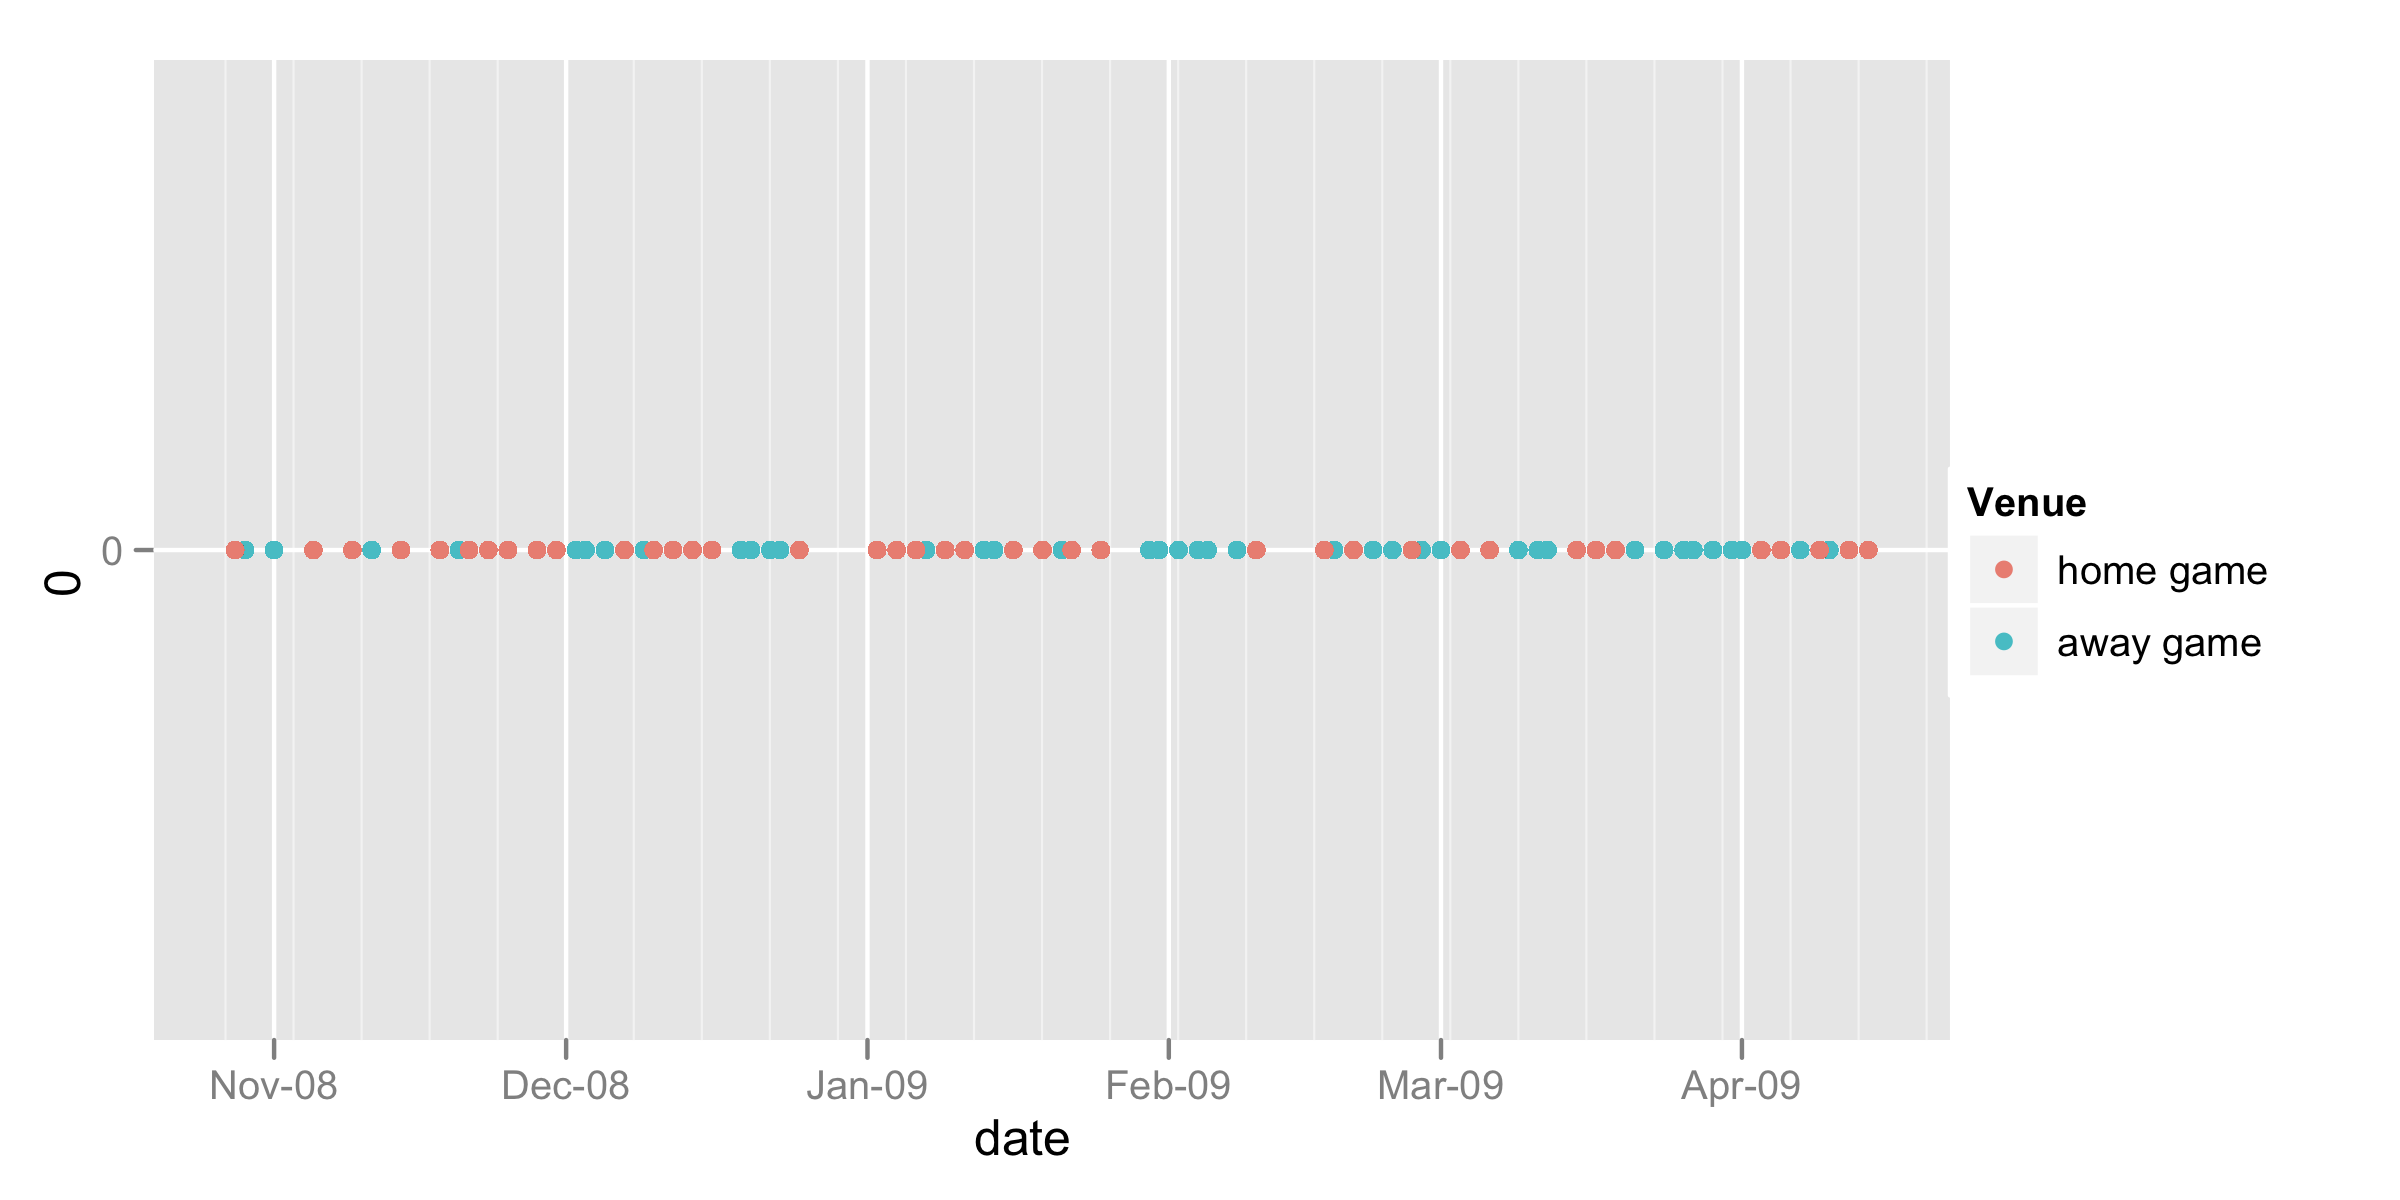
\includegraphics[width=\textwidth]{dates-points.png}        
  \caption{Home games and away games appear to occur in clusters.}
  \label{fig:games-date}
\end{figure}

Figure~\ref{fig:games-date} shows that games are played continuously throughout the season with a few short breaks. The frequency of games seems lower at the start of the season and games appear to be grouped into clusters of home games and away games. The tick marks and breaks on the x axis are automatically generated by the \pkg{lubridate} method \code{pretty.dates()}.

Next we will examine how Lakers games are distributed throughout the week. We use the \code{wday()} command to extract the day of the week of each date.

\begin{CodeInput}
R> qplot(wday(date, label = TRUE, abbr = FALSE), data = lakers, 
    geom = "histogram")
\end{CodeInput}

\begin{figure}[htpb]
  \centering    
    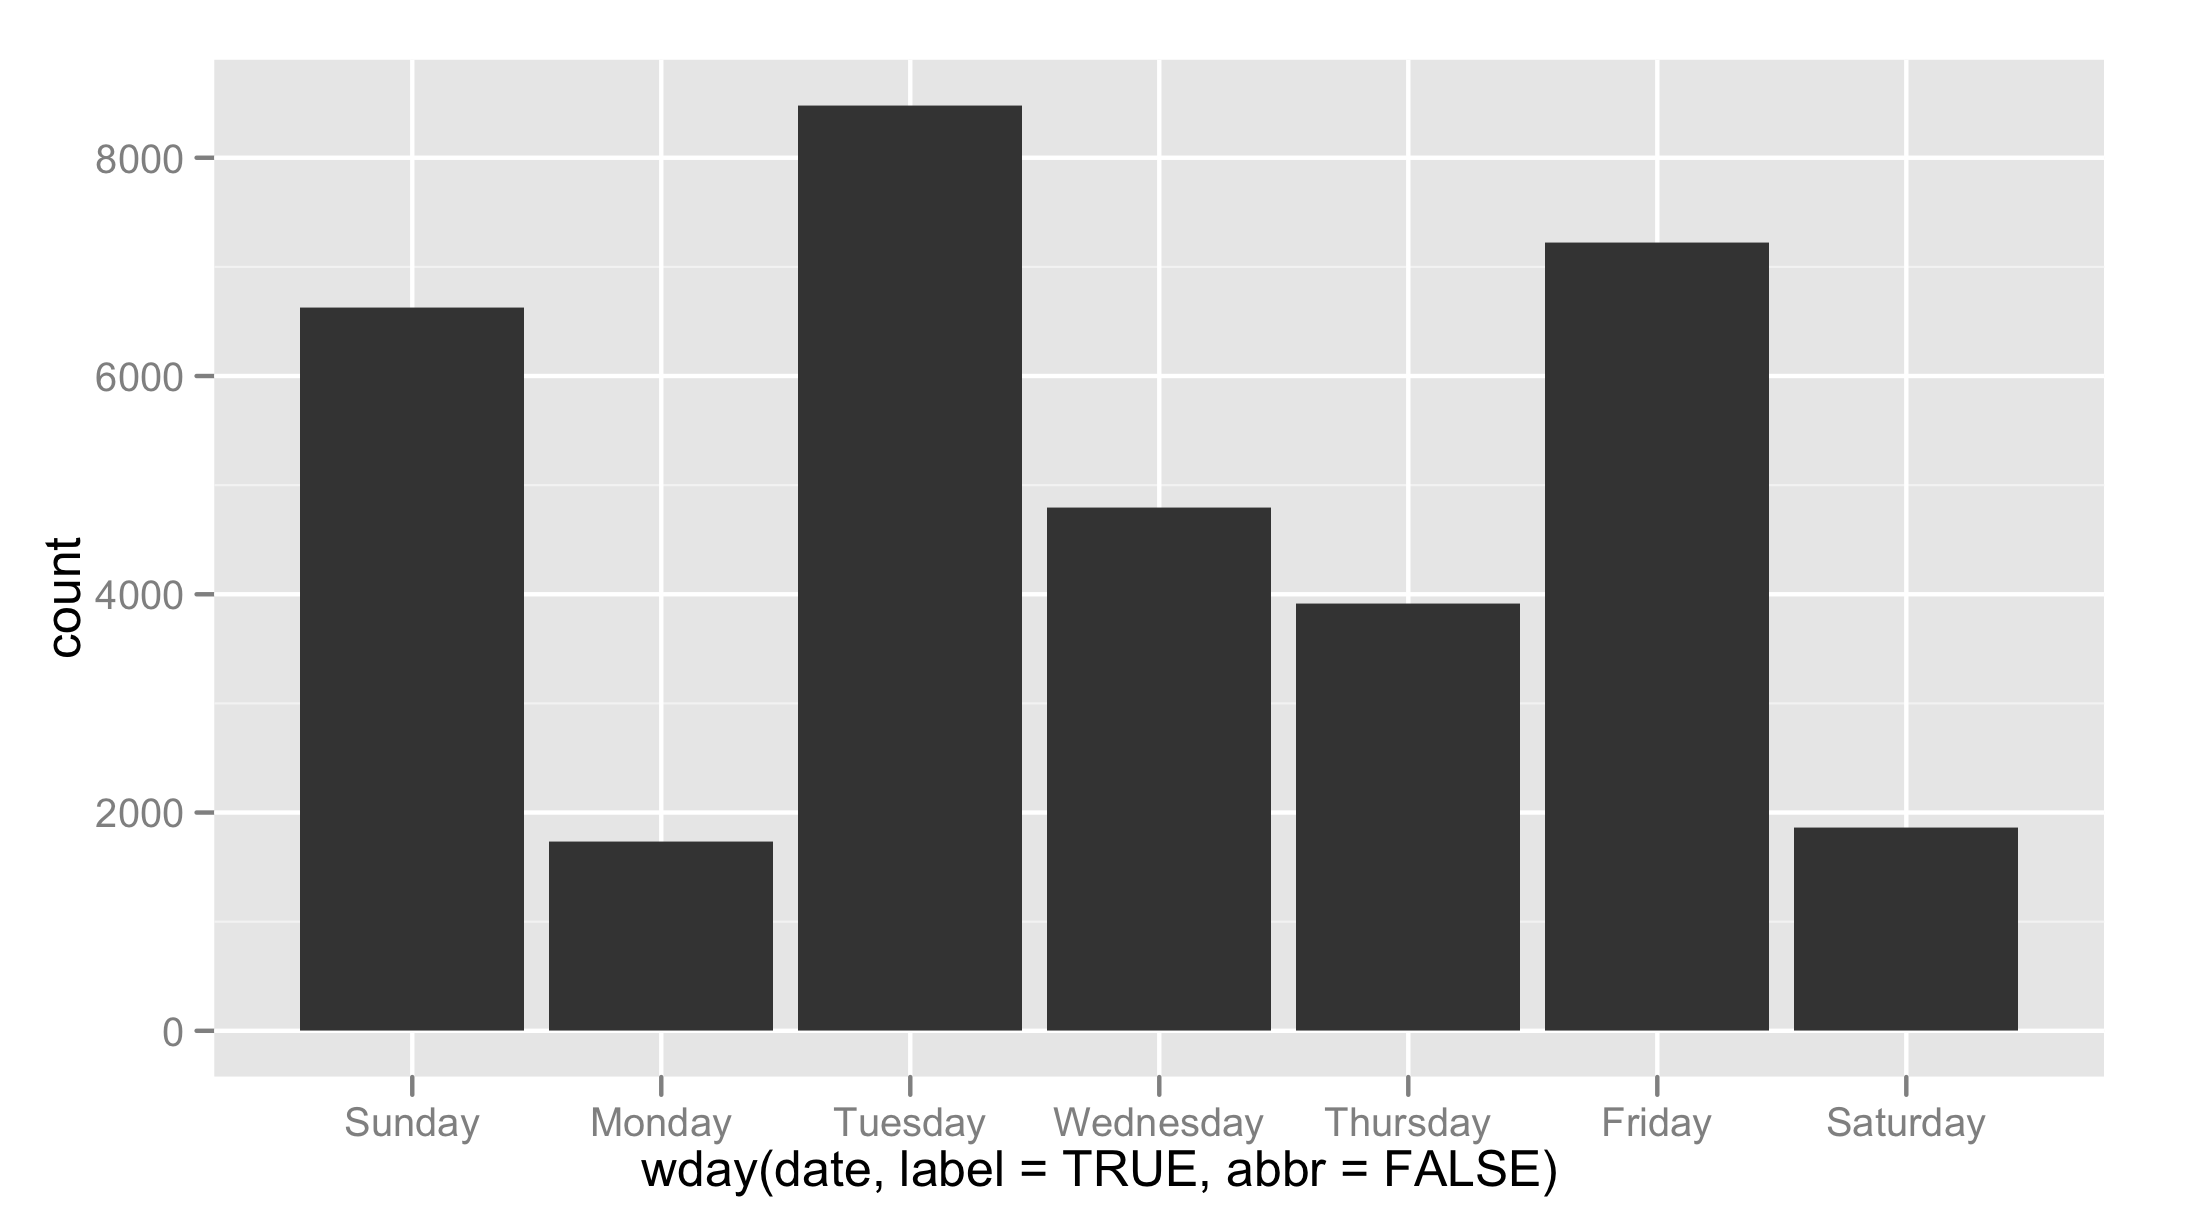
\includegraphics[width=\textwidth]{weekdays-histogram.png}     
  \caption{More games occur on Tuesdays than any other day of the week.}
  \label{fig:games-days}
\end{figure}


The frequency of basketball games varies throughout the week (Figure~\ref{fig:games-days}). Surprisingly, the highest number of games are played on Tuesdays.

Now we look at the games themselves. In particular, we look at the distribution of plays throughout the game. The \code{lakers} data set lists the time that appeared on the game clock for each play. These times begin at 12:00 at the beginning of each period and then count down to 00:00, which marks the end of the period. The first two digits refer to the number of minutes left in the period. The second two digits refer to the number of seconds.

The times have not been parsed as date-time data to \proglang{R}. It would be difficult to record the time data as a date-time object because the data is incomplete: a minutes and seconds element are not sufficient to identify a unique instant of time. However, we can store the minutes and seconds information as a \emph{\code{period}} object, as defined in Section~\ref{sec:periods}, using the \code{ms()} parse function.

\begin{CodeInput}
R> lakers$time <- ms(lakers$time)
\end{CodeInput}

Since periods have relative lengths, it is dangerous to compare them to each other. So we should next convert our periods to \emph{durations}, which have exact lengths.

\begin{CodeInput}
R> lakers$time <- as.duration(lakers$time)
\end{CodeInput}

This allows us to directly compare different durations. It would also allow us to determine exactly when each play occurred by adding the duration to the \emph{instant} the game began. (Unfortunately, the starting time for each game is not available in the data set). However, we can still calculate when in each game each play occurred. Each period of play is 12 minutes long and overtime---the 5th period---is 5 minutes long. At the start of each period, the game clock begins counting down from 12:00. So to calculate how much play time elapses before each play, we subtract the time that appears on the game clock from a duration of 12, 24, 36, 48, or 53 minutes (depending on the period of play). We now have a new duration that shows exactly how far into the game each play occurred.

\begin{CodeInput}
R>lakers$time <- dminutes(c(12, 24, 36, 48, 53)[lakers$period]) - lakers$time
\end{CodeInput}

We can now plot the number of events over time within each game (Figure~\ref{fig:plays}). We can plot the time of each event as a duration, which will display the number of seconds into the game each play occurred on the x axis,

\begin{CodeInput}
R> qplot(time, data = lakers, geom = "histogram", binwidth = 60)
\end{CodeInput}

or we can take advantage of \code{pretty.date()} to make pretty tick marks by first transforming each duration into a date-time. This helper function recognizes the most intuitive binning and labeling of date-time data, which further enhances our graph. To change durations into date-times we can just add them all to the same date-time. It doesn't matter which date we chose. Since the range of our data occurs entirely within an hour, only the minutes information will display in the graph.

\begin{CodeInput}
R> lakers$minutes <- ymd("2008-01-01") + lakers$time
R> qplot(minutes, data = lakers, geom = "histogram", binwidth = 60)
\end{CodeInput}

\begin{figure}[htpb]
  \centering
  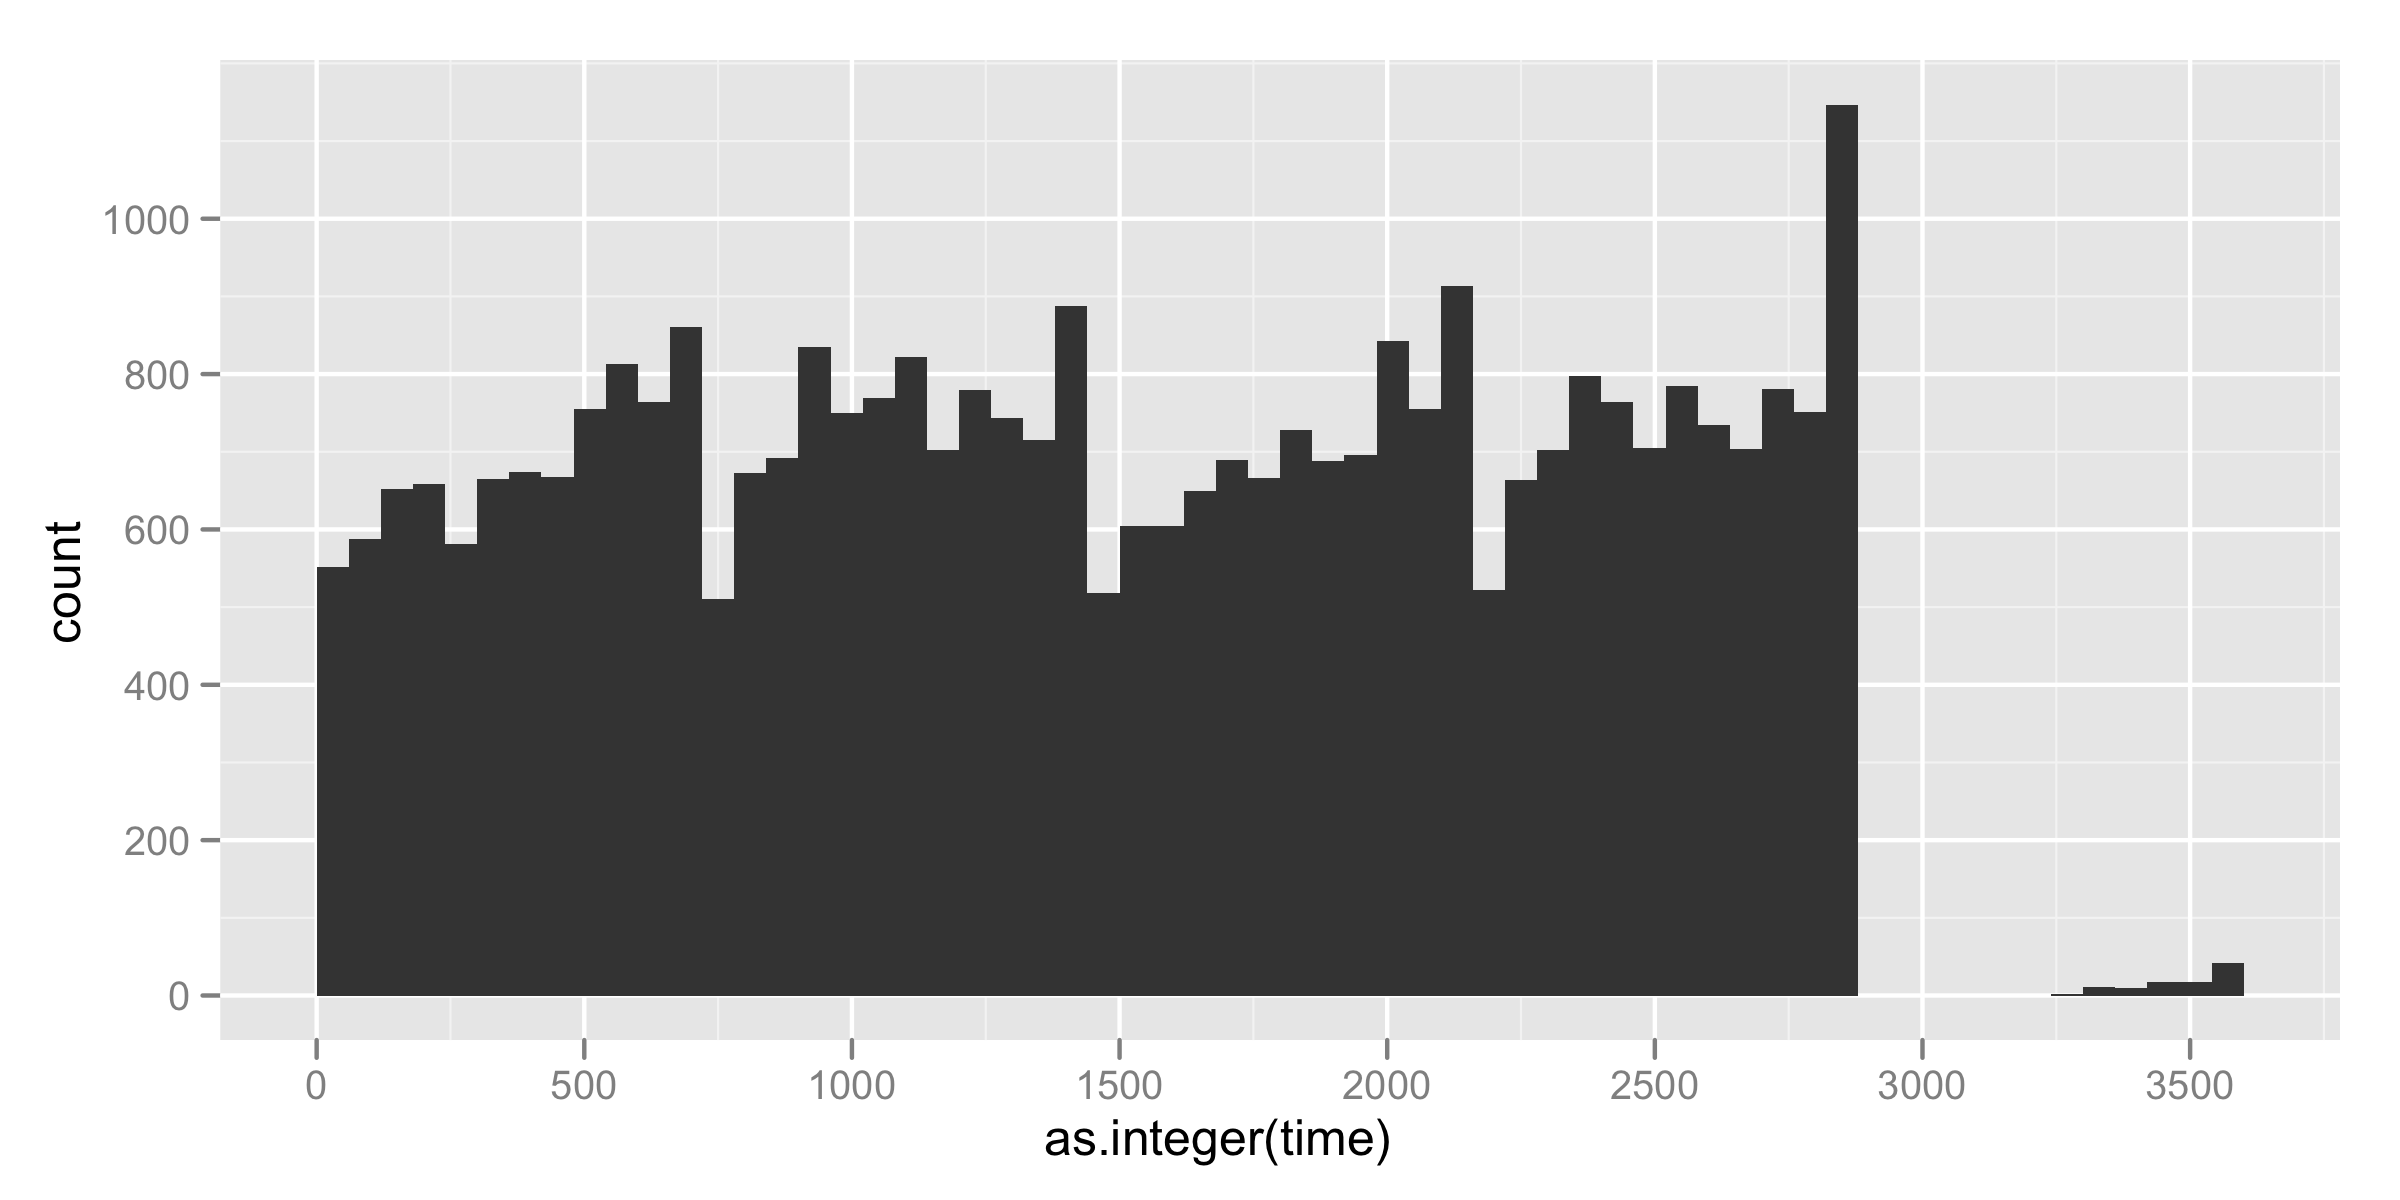
\includegraphics[width=0.49\textwidth]{play-time-histogram.png}        
  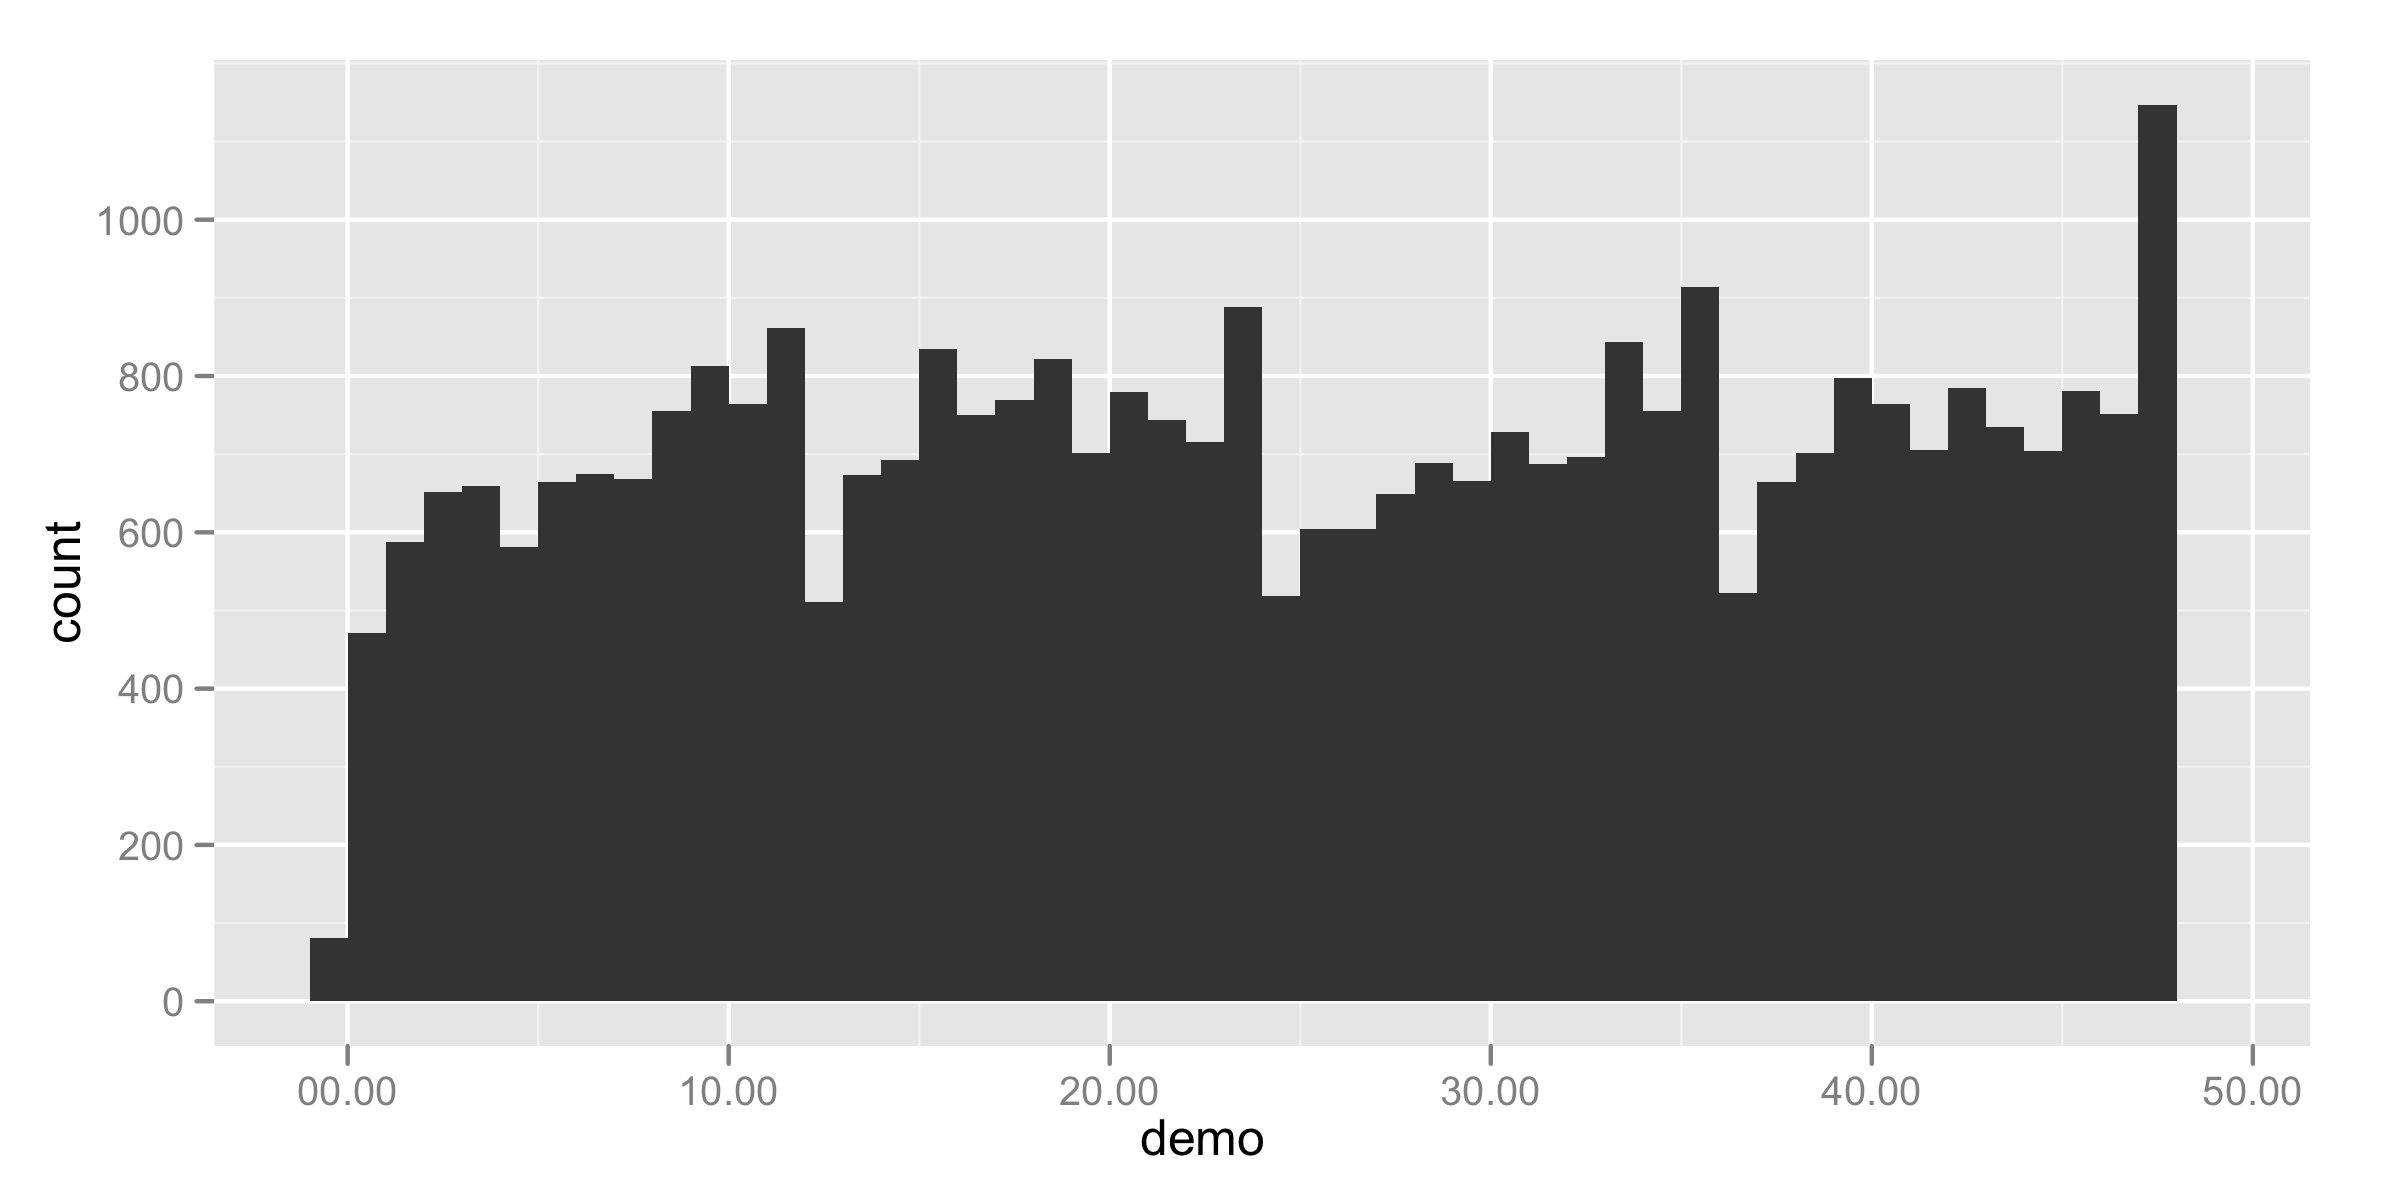
\includegraphics[width=0.49\textwidth]{play-time-histogram2.png} 
  \caption{The graph on the left displays seconds on the x axis. The graph on the right uses a more intuitive division with minutes.}
  \label{fig:plays}
\end{figure}

We see that the number of plays peaks within each of the four periods and then plummets at the beginning of the next period, Figure~\ref{fig:plays}. The most plays occur in the last minute of the game. Perhaps any shot is worth taking at this point or there's less of an incentive not to foul other players. Fewer plays occur in overtime, since not all games go to overtime.

Now lets look more closely at just one basketball game: the game played against the Boston Celtics on Christmas of 2008. We can quickly model the amounts of time that occurred between each shot attempt.

\begin{CodeInput}
R> game1 <- lakers[lakers$date == ymd("20081225"),]
R> attempts <- game1[game1$etype == "shot",]
\end{CodeInput}

The waiting times between shots will be the timespan that occurs between each shot attempt. Since we have recorded the time of each shot attempt as a duration (above), we can record the differences by subtracting the two durations. This automatically creates a new duration whose length is equal to the difference between the first two durations.

\begin{CodeInput}
R> attempts$wait <-  c(attempts$time[1], diff(attempts$time))
R> qplot(as.integer(wait), data = attempts, geom = "histogram", binwidth = 2)
\end{CodeInput}

\begin{figure}[htpb]
  \centering
  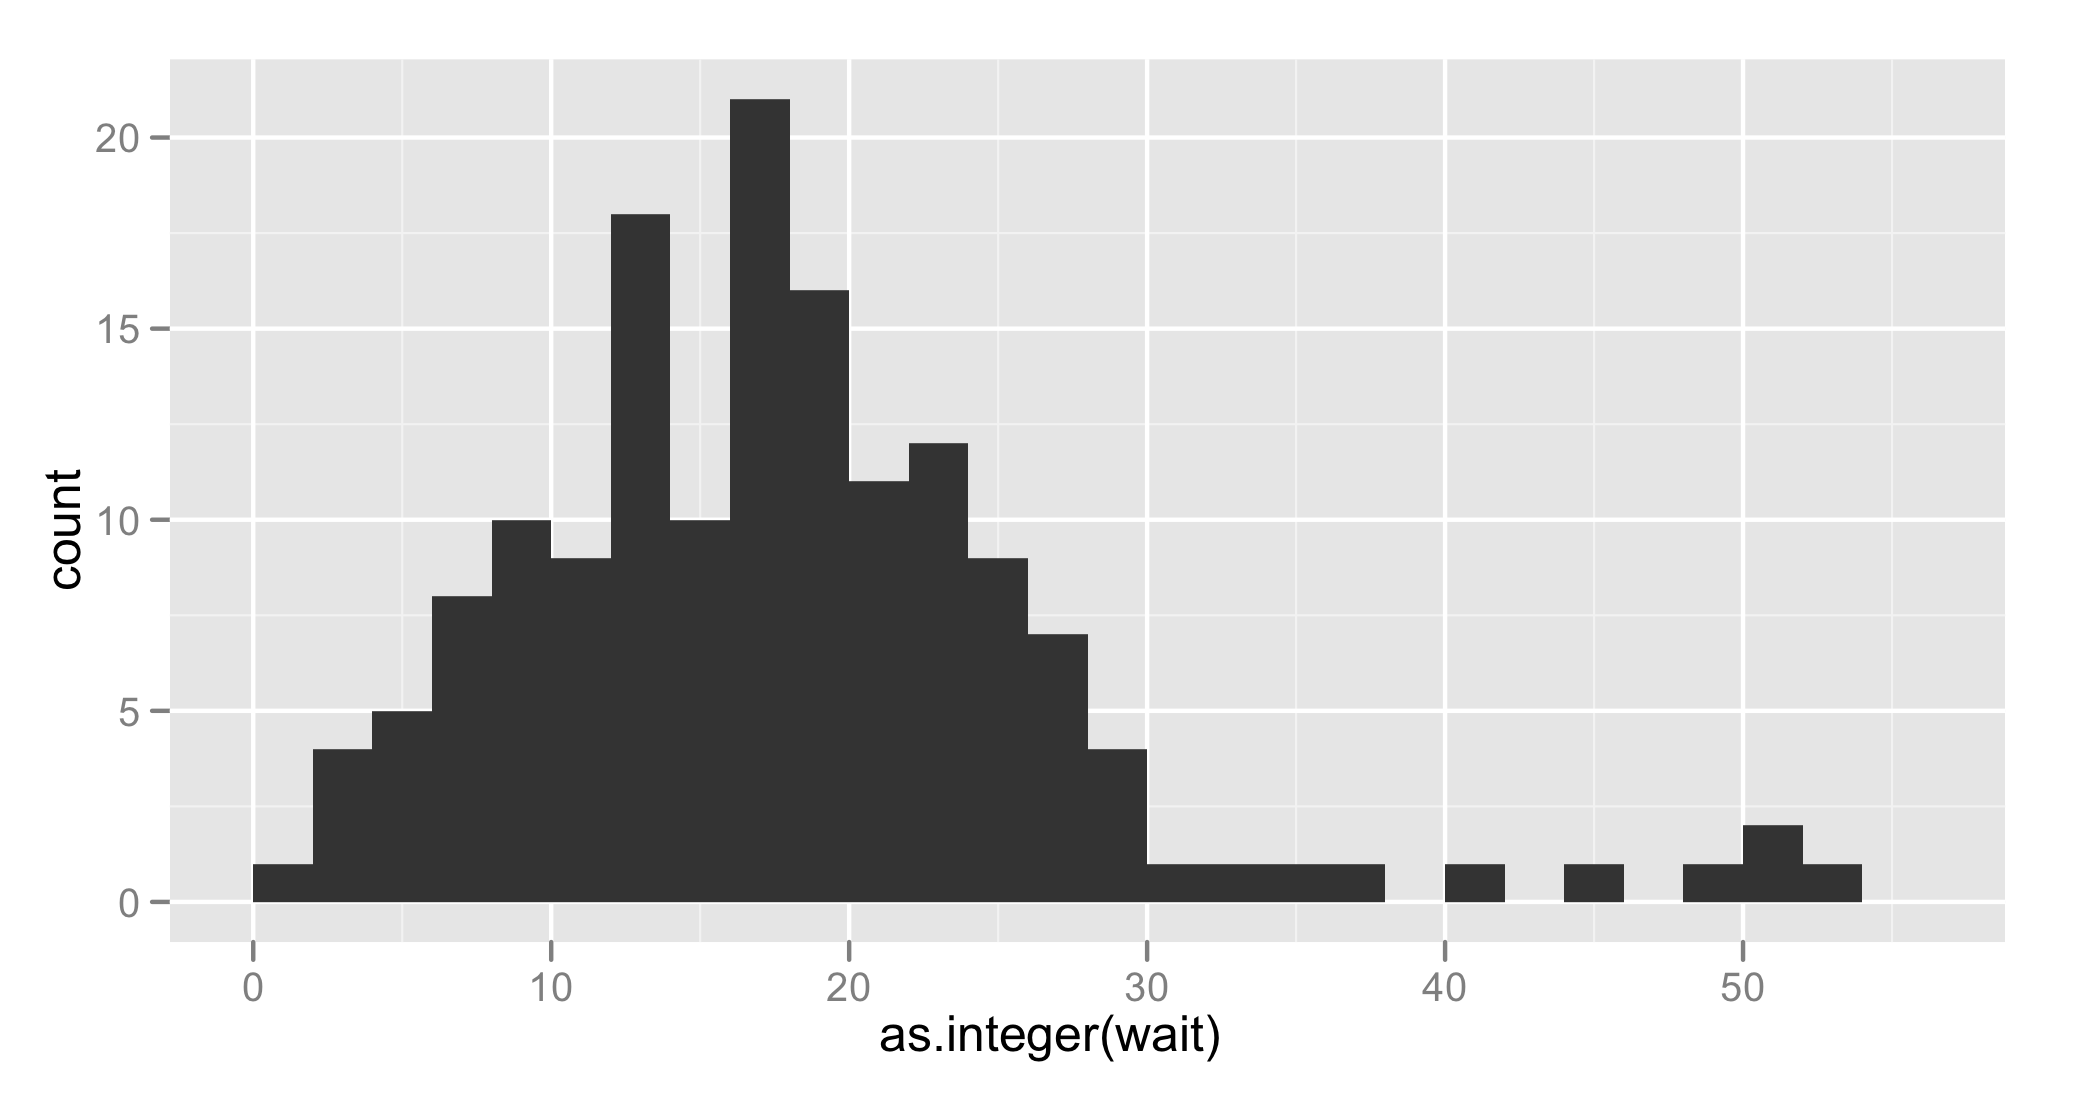
\includegraphics[width=\textwidth]{wait-histogram.png}        
  \caption{Wait times between shot attempts rarely lasted more than 30 seconds.}
  \label{fig:waits}
\end{figure}

Rarely did 30 seconds go by without at least one shot attempt, but on occasion up to 50 seconds would pass without an attempt.

We can also examine changes in the score throughout the game. This reveals that though the game was eventful, the Lakers maintained a lead for the most of the game, Figure~\ref{fig:scores}. Note: the necessary calculations are made simpler by the \code{ddply()} function from the \pkg{plyr} package, which \pkg{lubridate} automatically loads.

\begin{CodeInput}
R> game1_scores <- ddply(game1, "team", transform, score = cumsum(points))
R> game1_scores <- game1_scores[game1_scores$team != "OFF",]
R> qplot(ymd("2008-01-01") + time, score, data = game1_scores, 
    geom = "line", colour = team)
\end{CodeInput}

\begin{figure}[htpb]
  \centering
  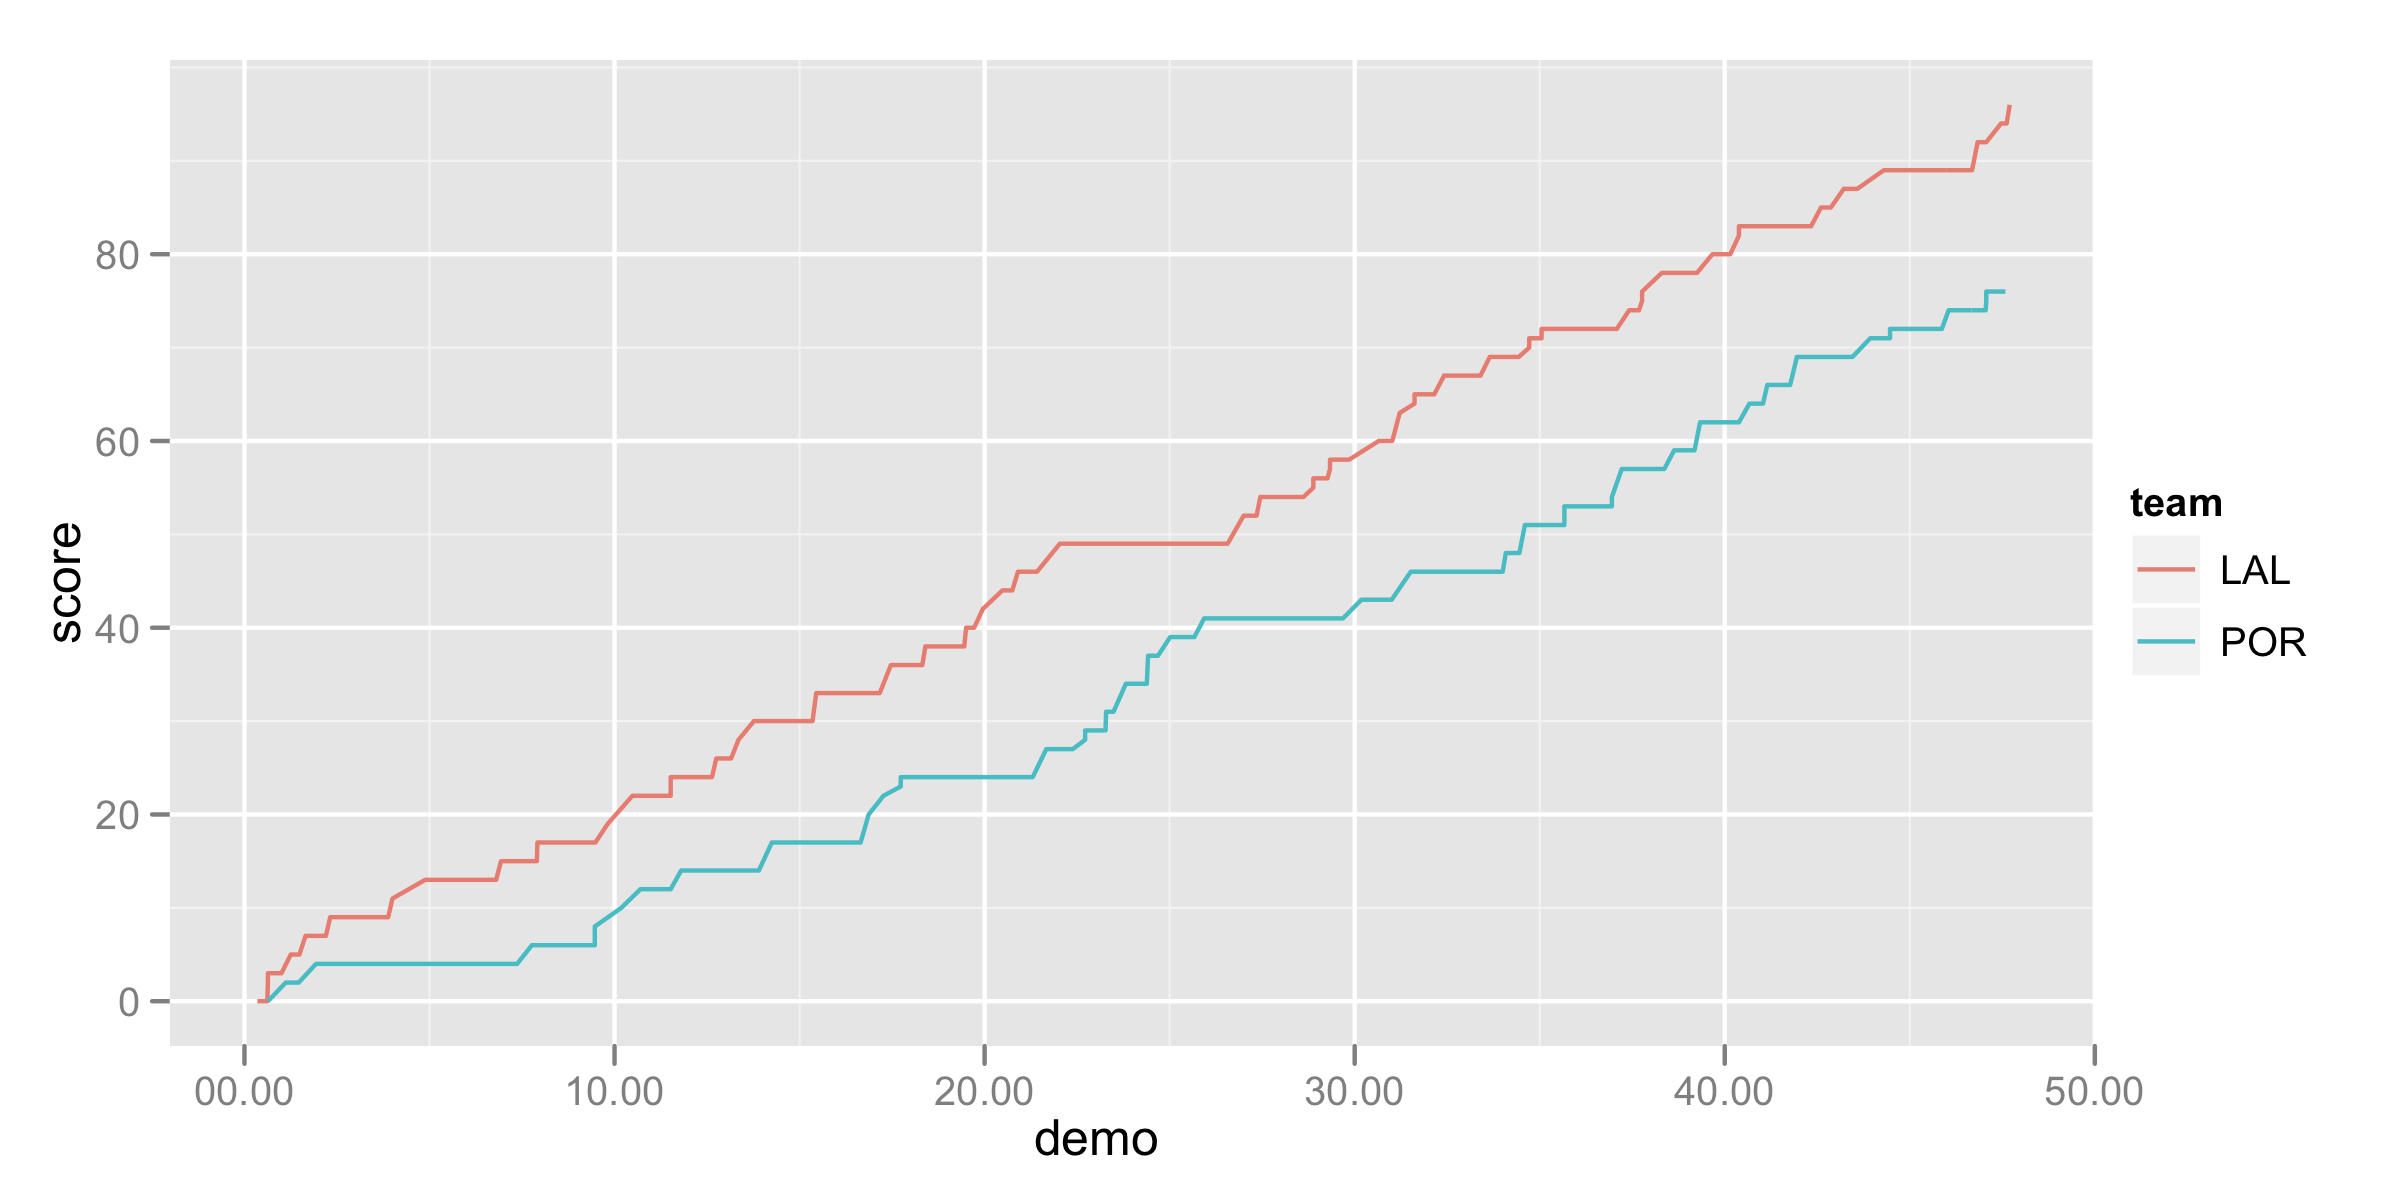
\includegraphics[width=\textwidth]{score-comparison.png}        
  \caption{The lead changed between the Lakers and Celtics numerous times during the game.}
  \label{fig:scores}
\end{figure}


\section{Conclusion}
Date-times create technical difficulties that other types of data do not. They must be specifically identified as date-time data, which can be difficult due to the overabundance of date-time classes. It can also be difficult to access and manipulate the individual pieces of data contained within a date-time. Arithmetic with date-times is often appropriate, but must follow different rules than arithmetic with ordinal numbers. Finally, date-related conventions such as daylight savings time and time zones make it difficult to compare and recognize different moments of time.

Base \proglang{R} handles many of these difficulties, but not all. Moreover, base \proglang{R}'s date-time methods can be complicated and confusing. \pkg{lubridate} makes it to easier to work with date-time data in \proglang{R}. The package provides a set of standard methods for most common date-time classes. These methods make it simple to parse, manipulate, and perform calculations with date-time objects. By implementing the time concepts pioneered by projects such as \pkg{Joda Time} and \pkg{Boost.Date\_Time}, \pkg{lubridate} helps researchers perform precise calculations as well as model tricky time-related processes. \pkg{lubridate} also makes it simple to switch between time zones and to use or ignore daylight savings time.

Future work on the \pkg{lubridate} package will develop methods for handling partial dates and for modeling recurrent events, such as stock market opening times, business days, or street cleaning hours. In particular, we hope to create methods for \proglang{R} that work with reoccurring temporal date patterns, which were introduced by \citet{fowler} and have been implemented in \proglang{Ruby} by the \proglang{runt} project \citep{runts}.

\section*{Acknowledgements}
We would like to thank the National Science Foundation. This work was supported by the NSF VIGRE Grant, number  DMS-0739420.


\bibliography{lubridate}


\end{document}
